\chapter{Results}

% What I want to say
%     - we see that there are differences between tokenizers on the metrics
%         - tokenizer method influences vocabulary allocation
%              - algorithm, and even implementation
%              - definitely compare my unigram / huggingface unigram to show the difference
%         - alpha factor influences vocabulary allocation
%         - data size influences vocabulary allocation but converges
%         - tokenizer influences vocabulary overlap but 
%         - data size influences vocabulary overlap but also converges
%     - 
% now with the knowledge of differences, lets compare the Limi unigram, Limi bpe and tokmix
% we see that the metrics correlate with the downstream tasks. Although there are task-specific differences
% - therefore cpt, ar, jsd are good metrics for comparing tokenizers

% - we can see that all balancing methods do influence the quality of the tokenizers on languages
% - we observe that all balancing methods produce similar improvements on lowresource
% - we check this by comparing the balancing methods on downstream and we do not see any significant differences between them. We do see improvements over the strong baseline in some cases.
% - therefore we can conclude that balancing does influence NER and POS tagging although with the comparison to alpha0.3, the improvements are very small

In this chapter, we present \xxx{our theoretical findings} and the results of our experiments. First we validate the usefulness of our proposed vocabulary allocation and vocabulary overlap metrics. \xxx{We do this on a theoretical level by analytically contrasting our metrics to existing metrics used in the literature. Then, } We do this by training three tokenizers using the Huggingface Tokenizers library and assessing whether they differ in the metrics we propose. We see that there are significant differences between the three tokenizers. Then we look at how these differences manifest, when we use these tokenizers to train otherwise identical multilingual models. We observe that the differences in tokenizers are reflected in the learned representations of the models. Especially when considering word-level downstream tasks, the learned contextualized representations are better when the tokenizer segments the text into longer tokens (high characters per token), when the tokenizer allocates tokens more uniformly (high average rank) and when there is less overlap between the languages (high Jensen-Shannon divergence).

Then we switch to the original Sentencepiece library, which is used in the related work we replicate \cite{conneau_unsupervised_2020,chung_improving_2020,zheng_allocating_2021,liang_xlm-v_2023}. We see that there are differences in the implementation of the Unigram and BPE algorithms between the two libraries and that the Huggingface library yields subpar Unigram tokenizers. We further assess other factors that influence the tokenizers quality, such as the total training data size, the language imbalance and size of the alphabet. We observe that we need around 100k-1M lines per language to train a good, multilingual tokenizer. The language imbalance does influence the per-language metrics heavily and the alphabet size does affect the number of UNK tokens but does not have a significant influence on the rest of the metrics if we stay in the range of 1000-5000 characters. We do this assessment to be better able to choose and fix the best parameters for the final set of experiments.

Finally, we replicate the works of \citet{chung_improving_2020,zheng_allocating_2021,liang_xlm-v_2023} and create several variations of their tokenizers that aim to improve the text segmentations especially for the low-resource languages. We carefully compare these replicated tokenizers with the traditional method of training Sentencepiece Unigram tokenizers on a joint, multilingual corpus. 

While the beforementioned authors do compare their methods to the standard tokenizer training, the crucial difference in our methodology is that we compare their replicated language-balancing methods with the vanilla Sentencepiece tokenizer trained on a \textbf{balanced} multilingual dataset. We find that when compared to this stronger, yet simple baseline, the balancing approaches do not yield significant improvements on our proposed tokenizer metrics per-language nor in overall.

We then validate our findings by training a second batch of masked language models that differ only in the tokenizer used. We choose the best performing balancing method of \citet{chung_improving_2020} and compare it with Sentencepiece Unigram tokenizers trained on balanced and unbalanced data. We observe that both the Chung method and balanced Unigram improve the language modeling capabilities over the unbalanced baseline on the word-level tasks while having no impact in the sentence-level task. On the other hand, we do not observe significant differences between the Chung method and the simple baseline of training the tokenizer on a balanced set which is in line with our previous assessment using only the tokenizer metrics. Our findings suggest that in our scaled down setting of 20 languages and 120k vocabulary size, the simpler method of training a tokenizer on a joint, balanced corpus is sufficient to create a good multilingual vocabulary that represents all languages well.

\section{Analytical comparison of the metrics}

\xxx{- move the comparison of the metrics here}

\section{The influence of tokenizer metrics on the language representation quality}
\label{sec:influence_of_metrics}

In this section, we present some of the results from \citet{limisiewicz_tokenization_2023}. We empirically establish that the metrics we propose are useful for assessing the differences between tokenizers. We also show that the differences in tokenizers are reflected in the learned representations of the models. 

% We train three distinct tokenizers --- Huggingface Unigram, Huggingface BPE and TokMix using the Huggingface Tokenizers library. The training data is the CC100 corpus sampled with the smoothing factor $\alpha=0.25$ which corresponds to the XLM-R tokenizer (there $\alpha=0.3$). For all tokenizers we choose the default  In the \ref{tab:20l_metrics} we see the overall macro average metrics for the three tokenizers. 

\begin{table}
\caption{In the first batch of experiments, we compare the Huggingface Unigram, Huggingface BPE, and our TokMix method based on merging Huggingface Unigram tokenizers. Huggingface Unigram has significantly lower vocabulary allocation scores ($-0.4$ CPT and $-153$ AR) than BPE and TokMix. This means that Unigram uses shorter tokens and the capacity of the vocabulary is used less uniformly. Moreover, the vocabulary has more overlap (JSD decrease by $-0.03$) between the languages for Unigram.  The scores are macro averages over all languages, computed over a holdout portion of the CC100 corpus. We sample 10k lines from each language which we have empirically found to be enough to get representative results.}
\label{tab:20l_metrics}
\begin{tabular}{lrrrrr}
\toprule
Tokenizer & Alphabet & \# UNKs & CPT & AR & JSD \\
\midrule
huggingface\_bpe\_alpha0.25 & 1000 & 14040.1 & 3.713 & 1253.7 & 0.783 \\
TokMix\_alpha0.25 & 2497 & 1203.2 & 3.691 & 1163.4 & 0.773 \\
huggingface\_unigram\_alpha0.25 & 12616 & 4.5 & 3.204 & 1010.5 & 0.745 \\
\bottomrule
\end{tabular}
\end{table}


In the \autoref{tab:20l_metrics} we see that the choice of the tokenization method largely influences the vocabulary allocation and overlap metrics. The Huggingface BPE tokenizer produces the most uniform allocation of tokens and the least overlap between languages. On the other hand, the Huggingface Unigram segments the text into shorter tokens and the average vocabulary overlap between all languages is much higher. The high overlap might be related to the low allocation as it is more likely that shorter tokens are shared between languages. Because we use the default Huggingface settings for the tokenizer training, the resulting tokenizers differ also in the vocabulary size. As we will discuss in \xxx{ref}, this difference is not sufficient to explain the difference between the tokenizers. Nevertheless the difference in alphabet size has an influence on the Chinese language. As we discuss in \citet{limisiewicz_tokenization_2023}, on the language level, the Unigram Tokenizer allocates more tokens to Chinese (as measured by the Average Rank metric) compared to the other methods. This is probably related to the alphabet size, where the majority of the low-occurence tokens might come from the less frequent logograms of the Chinese dictionary.

Next, we use the tokenizers from \autoref{tab:20l_metrics} and pretrain three masked language models with otherwise identical configuration and training data. We then evaluate the quality of the output representations of these models by probing the contextualized vectors against several tasks (XNLI, UD, POS, NER). We test the in-language and cross-lingual settings. The in-language setting are shown in \autoref{fig:pair_analysis_20L}.e show the relationship between our metrics and the downstream tasks. The probe performance is largely dependent on the tested language, to assess only the differences yielded by the use of different tokenizers, we center the per-language results on the mean across the three models. This way we can see only the improvements and deteriorations of the models compared to the mean. The metrics are centered in the same way. We can see that the differences between tokenizers are reflected in the representation quality. High CPT and AR metrics are correlated with better probe performance especially on the word-level tasks such as Part of speech tagging, Named entity recognition and Dependency labeling. Moreover the cross-lingual performance is also correlated with the JSD metric as shown in \autoref{fig:X_pair_analysis_20L}.

\xxx{maybe I can actually get rid of the scatterplots and just show the correlation tables from the paper. The problem is the mixing of 6 langs and 20 langs which I do not explain here.}

All correlations are summarized in \autoref{tab:corr_in_lang_20l} and \autoref{fig:corr_x_lang_20l}. The length of the tokens has a strong positive influence on POS, dependency labeling, and NER results ($r > 0.65$), while it does not significantly affect NLI results. The correlation between the average rank NER scores is weaker but still significant. Moreover, it is significantly correlated with XNLI accuracy with a medium coefficient $r = 0.56$. 

\xxx{what to do with JSD, in paper we present the 6 lang experiments. Here I wanted to keep things simple and focus on the 20 lang experiments. But it seems that for 20 langs the influence of JSD is actually positive for NER and there is $\approx 0$ influence on XNLI. }

Note that in this results section we have included only a part of the experiments from our paper \citet{limisiewicz_tokenization_2023}. Namely we focus only on the experiments that are based on the same 20 languages as the rest of the thesis. For our purposes we focus only on the more general conclusions. We refer the reader to the original paper for the full set of experiments, where we additionaly discuss in more detail which tasks are more affected by which properties of the tokenizers.

% Firstly, we see that the default settings of the Huggingface tokenizers produce very different alphabet sizes and in turn affect the UNK rate. As we will see later, this does not affect the metrics significantly.


\begin{figure}[H]
    \centering
    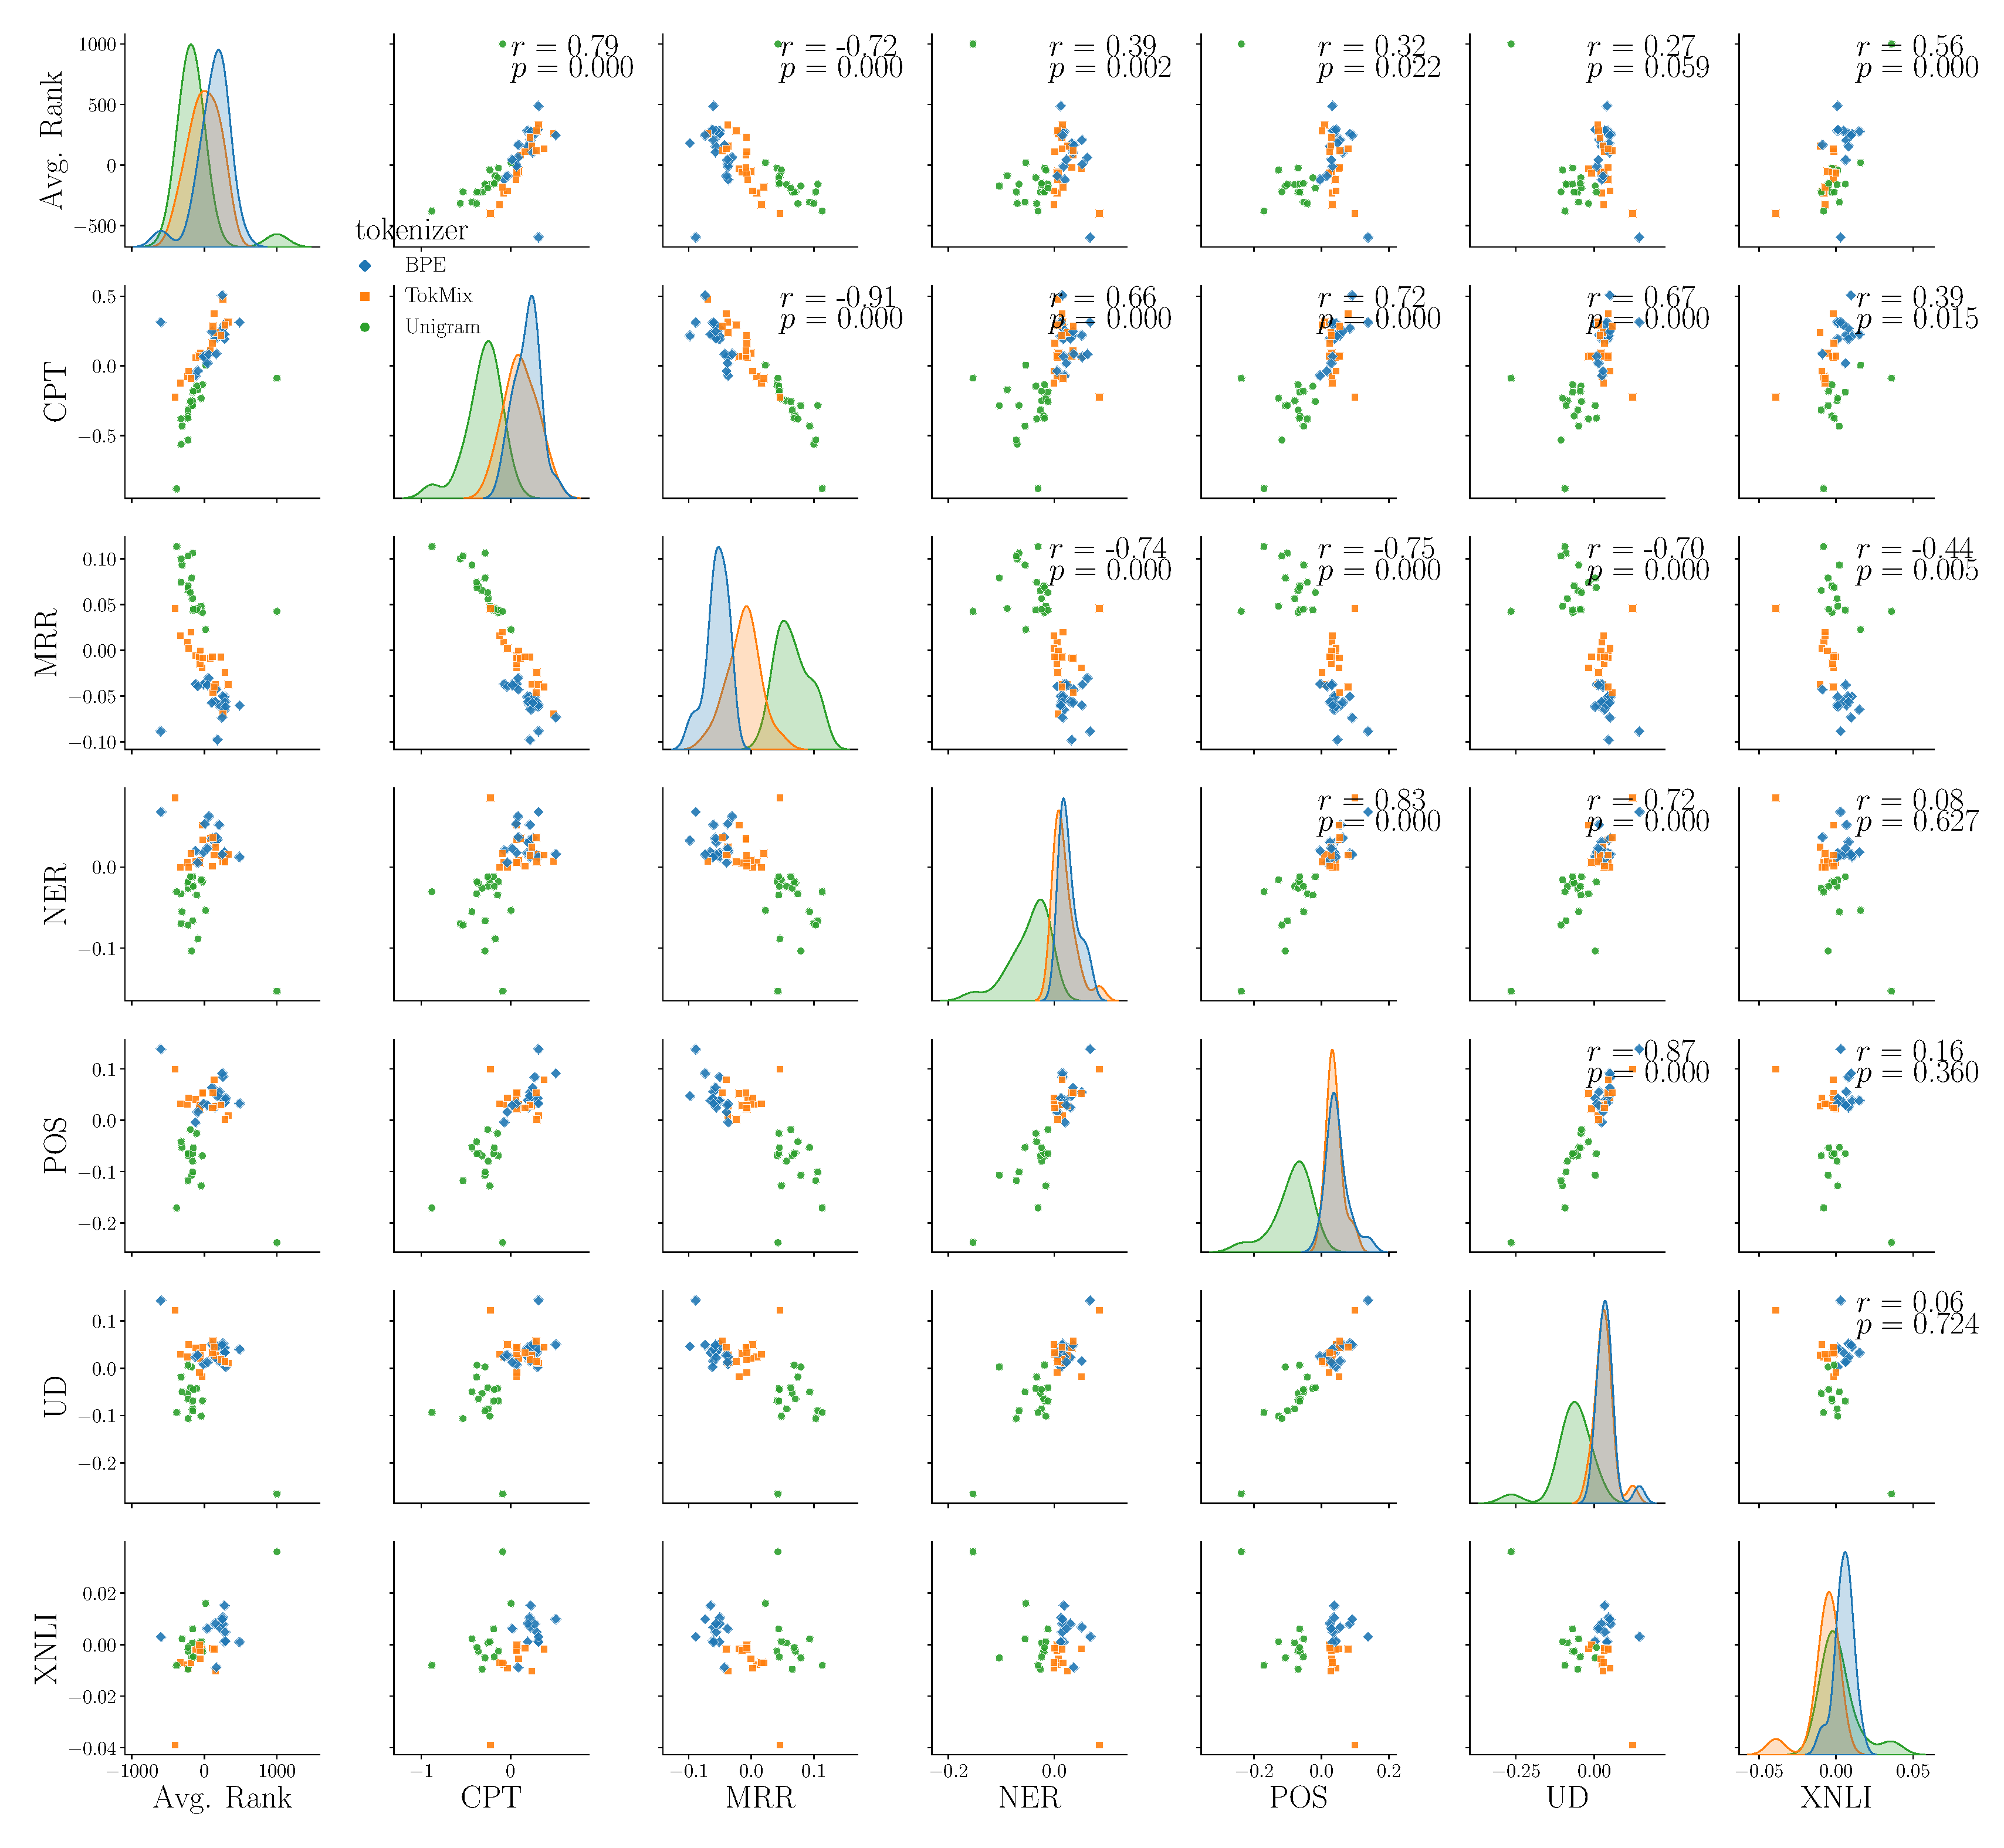
\includegraphics[width=\textwidth]{paper/figures/pair_analysis_20L.pdf}
    \caption{We compare the tokenizer metrics against the contextualized representation quality. For each tokenizer we pretrain a masked language model, freeze it and train a linear probe for each task and each of the available languages. We observe high spearman correlation between CPT and the word-level tasks (NER, POS, UD) and high correlation between AR and the sentence-level task XNLI. This suggests that our vocabulary allocation metrics are good indicators of the tokenizers quality and higher vocabulary allocation leads to better downstream performance. Each data point corresponds to an average result over three seeds of probe training and evaluating on one of the languages. The results for each language are centered around the mean to account for the differences between languages.}
    \label{fig:pair_analysis_20L}
\end{figure}

\begin{figure}[H]
    \centering
    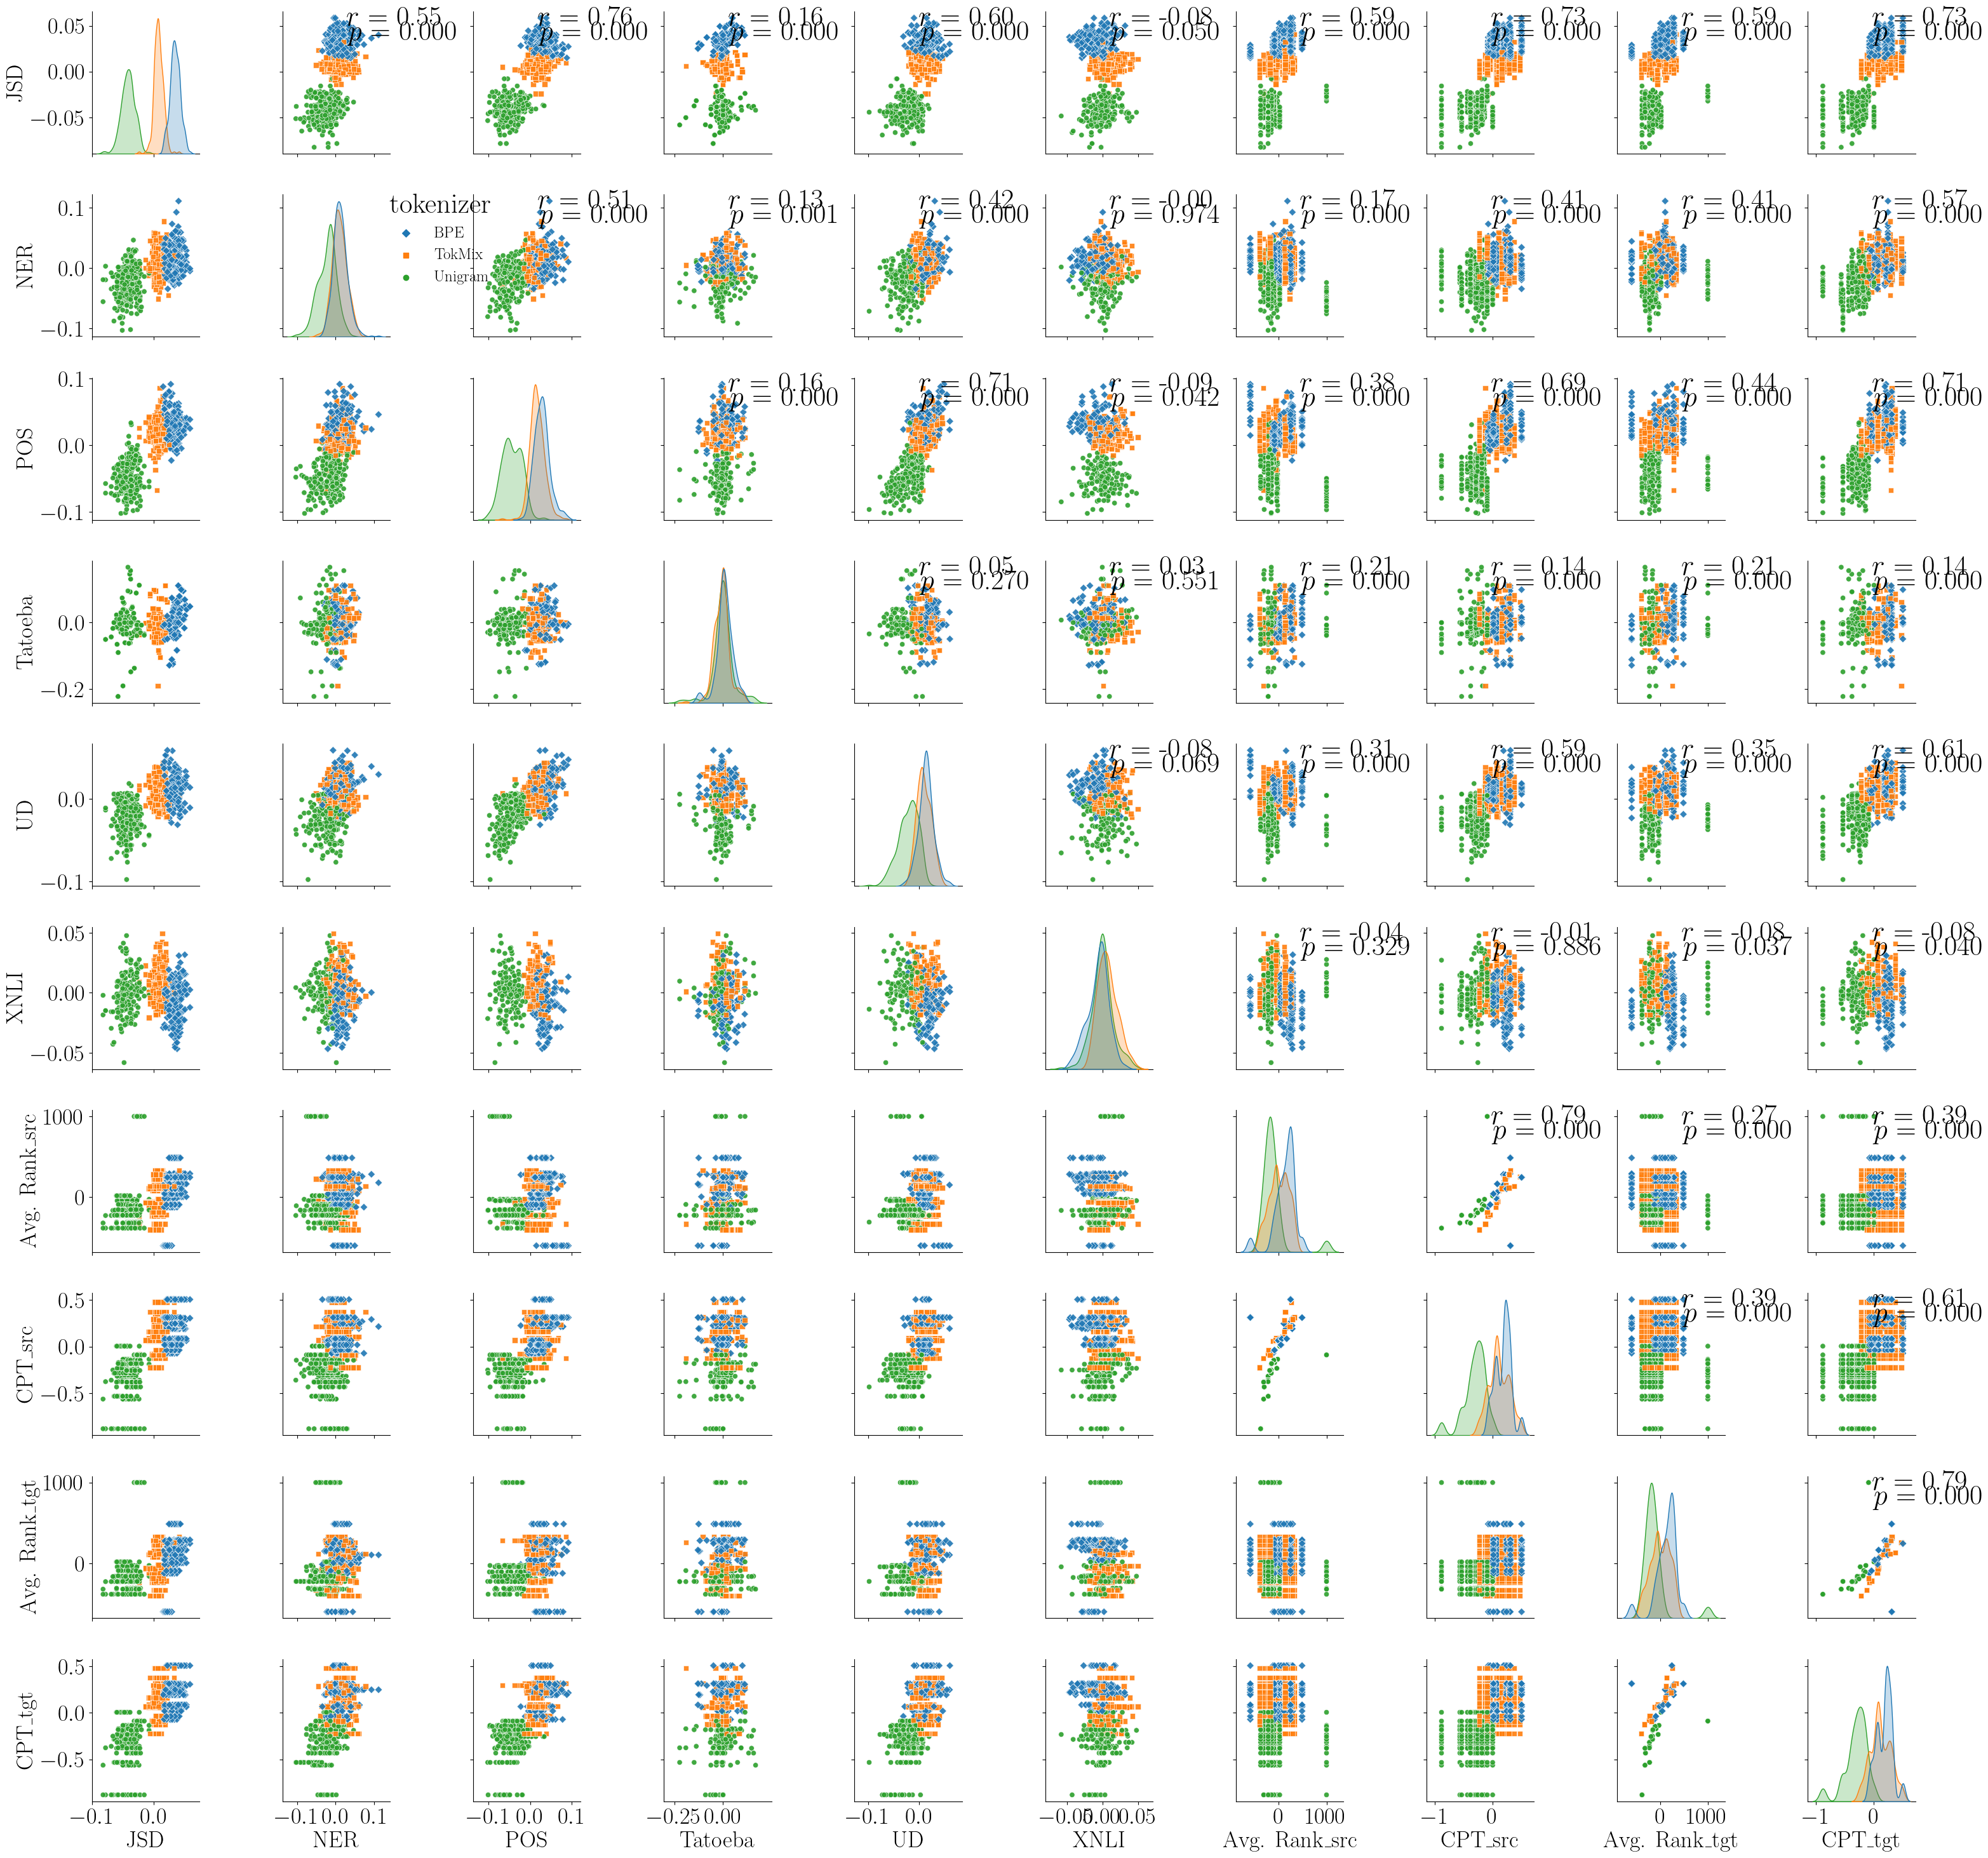
\includegraphics[width=\textwidth]{img/temp/X_pair_analysis_20L.png}
    \caption{We compare the tokenizer metrics against the cross-lingual performance of the models. For each tokenizer we pretrain a masked language model, freeze it and train a linear probe on each of the available languages. Then we evaluate the models on all languages the probe has \textbf{not} been trained on, assessing the cross-lingual properties of the model. Here we observe high correlation between JSD and the word-level tasks, especially the POS and UD. This suggests that less overlap (higher divergence) between the vocabularies of the languages leads to better cross-lingual performance for the word-level tasks.
    \xxx{remove the ar and cpt metrics?}} \xxx{For XNLI, we see low correlation with a marginal p-value.}
    \label{fig:X_pair_analysis_20L}
\end{figure}

\begin{table}
\centering

\begin{tabular}{lccc}
\toprule
 & \multicolumn{2}{c}{\bf{V. Allocation}} & \bf{MLM} \\
 & (AR) &  (CPT)  &  (MRR) \\
\midrule
CPT    &    \bf{0.790} &     - &  - \\
MRR    &  \bf{-0.723} &  \bf{-0.913} &  - \\
NER    &   \bf{0.394} &   \bf{0.657} &  \bf{-0.745} \\
POS    &     0.320 &   \bf{0.724} &  \bf{-0.754} \\
Dep l. &     0.266 &   \bf{0.675} &  \bf{-0.695} \\
NLI   &    \bf{0.56} &    0.388 &  \bf{-0.437} \\ 
\bottomrule
\end{tabular}
\caption{Spearman correlations between centered in-language task results and tokenizer measures. Statistically significant correlations ($p<0.01$) are bolded. Computed for 20 languages.}
\label{tab:corr_in_lang_20l}
\end{table}

\begin{figure}[H]
    \centering
    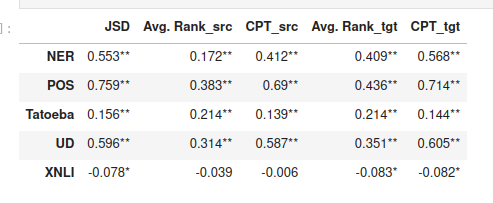
\includegraphics[width=\textwidth]{img/temp/corr_x_lang_20l.png}
    \caption{Correlations between task cross-lingual transfer results and tokenization measures."Stars denote statistical significance: (* coresponeds to $p<0.05$ and ** to $p<0.01$).\xxx{remove the ar and cpt metrics? Merge with the previous correlation table?}}
    \label{fig:corr_x_lang_20l}
\end{figure}

% ---------

\section{The choices that influence the tokenizers quality}

\subsection{Implementation}
\label{sec:implementation}

\begin{table}
\caption{In this table, we compare the Huggingface and Sentencepiece implementations of the Unigram and BPE algorithms. As shown, the Huggingface Unigram tokenizer is a clear outlier in terms of all metrics. We can see that this is a problem in the implementation as the corresponding Sentencepiece \textit{unigram\_alpha0.3} scores much higher. As we will explore in \ref{tab:coverage_influence}, the different alphabet size does not influence the metrics enough to explain the difference. \xxx{here I can add an experiment with the same alphabet size, to be able to skip the reference} Interestingly, we found that the BPE implementation (\textit{huggingface\_bpe\_alpha0.25}) is better in Huggingface than in Sentencepiece (\textit{bpe\_alpha0.25}).}
\label{tab:hugg_vs_sentpiece}
\begin{tabular}{lrrrrr}
\toprule
Tokenizer & Alphabet & \# UNKs & CPT & AR & JSD \\
\midrule
huggingface\_bpe\_alpha0.25 & 1000 & 14040.1 & 3.713 & 1253.7 & 0.783 \\
unigram\_alpha0.3 & 2666 & 923.5 & 3.702 & 1190.7 & 0.768 \\
bpe\_alpha0.25 & 1215 & 7235.6 & 3.666 & 1212.9 & 0.774 \\
huggingface\_unigram\_alpha0.25 & 12616 & 4.5 & 3.204 & 1010.5 & 0.745 \\
\bottomrule
\end{tabular}
\end{table}


As shown in the previous \autoref{sec:influence_of_metrics}, we observe that the Huggingface Unigram tokenizer leads to significantly worse metrics than the other tokenizers. We investigate this difference by turning to the original Sentencepiece implementation of the algorithm and running a comparable experiment with the different library. For comparison, we also train a comparable BPE tokenizer using the Sentencepiece. 

The results are presented in \autoref{tab:hugg_vs_sentpiece}. We see that the implementation has an effect on the tokenization and that the Sentencepiece Unigram tokenizers performs on par with the Huggingface BPE tokenizer. For this reason, we use the Sentencepiece implementation for the rest of the experiments.

\subsection{Data size}
\label{sec:data_size}

\begin{table}
\centering
\caption{We measure how much data is generally needed for the tokenizer training. We train handful of Sentencepiece Unigram tokenizers on different amounts of balanced multilingual data. We observe that after 100k-1M lines per language, the tokenizers converge to similar vocabulary allocation and overlap scores. The significance of this experiment is that we find out experimentally how much data is needed for the tokenizer training and we can use this information to make sure that we provide enough data for each language for the further experiments.}
\label{tab:data_size_influence}
\begin{tabular}{rrrrrr}
\toprule
 Lines per language &  Alphabet size &  Number of UNKs &      CPT &          AR &      JSD \\
\midrule
               1000 &           3598 &          520.35 & 3.301636 &  958.414048 & 0.765687 \\
              10000 &           4725 &          117.75 & 3.597563 & 1089.112498 & 0.765236 \\
             100000 &           5041 &           65.55 & 3.695797 & 1192.201089 & 0.767133 \\
            1000000 &           5079 &           62.60 & 3.702038 & 1204.659073 & 0.767357 \\
            1500000 &           5176 &           55.90 & 3.705119 & 1210.664835 & 0.767348 \\
            2000000 &           5180 &           56.35 & 3.705109 & 1212.489940 & 0.767327 \\
\bottomrule
\end{tabular}
\end{table}


We are interested in how much data is needed for the tokenizer training. For this experiment, we sample the same number of lines (1e3, 1e4, 1e5, 1e6, 1.5e6, 2e6 per language) for each language from the CC100 corpus. Then we train the Sentencepiece Unigram tokenizers on different amounts of data and compare the results in \autoref{tab:data_size_influence}. We see that the metrics improve with the amount of data, but the improvement is not substantial after 100k-1M lines per language. We use these results as a rule of thumb for the rest of the experiments and where possible, we use at least 100k but preferrably 1M lines per language for the rest of the experiments.

\subsection{Character coverage}
\label{sec:character_coverage}

\begin{table}
\caption{We check the tradeoff of including a large alphabet size. We train Sentencepiece Unigram tokenizers with a different target character coverage and observe the resulting alphabet size, number of UNKs and tokenizer metrics. We observe that the alphabet size grows with the coverage and the number of UNKs decreases, as expected. We observe that at both extremes of the character coverage parameter, the vocabulary allocation decreases. The results indicate that the alphabet size between 1000 and 5000 provides a good tradeoff between the number of UNKs and the allocation metrics, while including all characters in the alphabet does not come with a significant decrease in the allocation metrics (-0.05 CPT).}
\label{tab:coverage_influence}
\begin{tabular}{lrrrrr}
\toprule
Coverage & Alphabet & \# UNKs & CPT & AR & JSD \\
\midrule
98.0\% & 539 & 17386.5 & 3.631 & 1115.3 & 0.749 \\
99.5\% & 1136 & 7786.9 & 3.702 & 1173.1 & 0.765 \\
99.95\% & 2678 & 910.6 & 3.705 & 1196.7 & 0.768 \\
99.995\% & 4813 & 83.0 & 3.695 & 1188.7 & 0.769 \\
99.9995\% & 8226 & 10.2 & 3.678 & 1164.2 & 0.769 \\
100.0\% & 13658 & 1.9 & 3.650 & 1124.1 & 0.768 \\
\bottomrule
\end{tabular}
\end{table}


Because we observe the large difference in the alphabet size between Huggingface tokenizers (implied by the use of the default trainer settings of the library), we investigate the influence of this parameter on our tokenizer metrics. We train the Sentencepiece Unigram tokenizers with different character coverage (98\%, 99.5\%, 99.95\%, 99.995\%, 99.9995\%, 99.99995\% and 100.0\%) on balanced data sampled from CC100 with $\alpha=0.0$. and compare the results in \autoref{tab:coverage_influence}. The character coverage parameter determines, how many distinct Unicode characters are included in the vocabulary of the tokenizer. As expected, we see that there is a direct relationship between the character coverage, alphabet size and the number of unknown tokens in the validation set. We also see that our metrics are not largely affected by the alphabet size, as the alphabet accounts for at most 10\% of the whole vocabulary size 120\,000. The lowest vocabulary allocation metrics are on the extremes of the character coverage, where the alphabet size is either very small or very large. We assume that the small alphabet size leads to a large number of unknown tokens and the tokenizer is forced to segment words containing characters outside of the alphabet, as these unknown tokens might even be characters with diacritics. In the range of 1000-5000 alphabet size, we see that the metrics are not largely affected by the alphabet size. On the other extreme, the large alphabet size starts to take up a large portion of the vocabulary and the tokenizer might not have enough capacity to learn longer tokens. For later experiments, we use the Sentencepiece default character coverage of 99.95\%. When comparing tokenizers with different alphabet sizes, we are aware of the fact that the metrics might be affected by the alphabet size and we take this into account when interpreting the results.

\section{Tokenizer training with data imbalance}

\begin{table}
\caption{We train five Sentencepiece Unigram tokenizers on increasingly imbalanced multilingual dataset. We see that the macro averaged metrics decrease with the increasing imbalance, suggesting that on average, the tokenizer represents the languages less well.}
\label{tab:data_balance_metrics}
\begin{tabular}{lrrrrr}
\toprule
Tokenizer & Alphabet & \# UNKs & CPT & AR & JSD \\
\midrule
Unigram $\alpha$=0.0 & 2975 & 617.1 & 3.712 & 1212.9 & 0.767 \\
Unigram $\alpha$=0.3 & 2666 & 923.5 & 3.702 & 1190.7 & 0.768 \\
Unigram $\alpha$=0.5 & 2859 & 729.0 & 3.618 & 1143.8 & 0.769 \\
Unigram $\alpha$=0.7 & 2733 & 883.2 & 3.556 & 1107.1 & 0.770 \\
Unigram $\alpha$=1.0 & 2476 & 1286.3 & 3.442 & 1041.8 & 0.772 \\
\bottomrule
\end{tabular}
\end{table}


In this section, we present the tokenizers that become the baselines for comparing the related works we replicate. Our experiments with the data imbalance follow the original tokenizer training recipe from XLM-R and mBERT. The method is training the tokenizers on a corpus created by combining monolingual data in different proportions. On one extreme we have the $\alpha=1.0$, where all data available for each language is combined. On the other we have $\alpha=0.0$, where the data is sampled per-line from each language with the same probability. 

The contribution of our method is investigating how the language imbalance affects each language individually. Moreover, we investigate how the other proposed methods relate to all settings of $\alpha$, not only the most unbalanced settings of $\alpha=0.5 \textrm{ or } 0.7$.

For the data balancing experiment, we train 5 tokenizers on an increasingly imbalanced corpus with $\alpha = 0.0, 0.3, 0.5, 0.7, 1.0$ using the CC100 with 20 languages. For $\alpha = 0.0, 0.3, 0.5, 0.7$ we make sure to sample at least 100k lines per language as we have found this to be important in \autoref{sec:data_size}. We note that the data imbalance for $\alpha=1.0$ is so large, we needed to settle for 30k-70k training lines for the five least resourceful languages (ka, ur, te, mr, sw) because of memory constrants. We use the Sentencepiece Unigram tokenizer with the default settings. Specifically we use the default character coverage 99.95\%. We evaluate the tokenizers on a balanced validation set sampled from holdout portion of the CC100 corpus. 

The overall results with metrics macro averaged over the 20 languages are presented in \autoref{tab:data_balance_metrics}. The results demonstrate a clear disparity in the performance of the Sentencepiece Unigram, with training on balanced data leading to higher overall metrics than unbalanced data. The imbalance also affects the alphabet as it is possible to cover 99.95\% of the characters in the training data with smaller alphabet because of overrepresentation of few high-resource languages.

We explore the reason for the decreasing performance of the tokenizers trained on imbalanced data in \autoref{fig:data_balance_vs_allocation_per_lang}. We see that the vocabulary allocation metrics for the high resource languages (en, vi, ru, fr, es, th) are improving with the data imbalance. On the other hand, the low resource languages (ka, ur, te, mr, sw) are disproporionally more affected by the imbalance and their vocabulary allocation metrics are decreasing significantly. This suggests that the marginal benefit of adding more data to the high resource languages is lower than the incurred cost on the quality of tokenization for the low resource languages. We see this tradeoff in the \autoref{tab:data_balance_metrics} as a overall decrease in the average CPT and AR.

\begin{figure}[H]
    \centering
    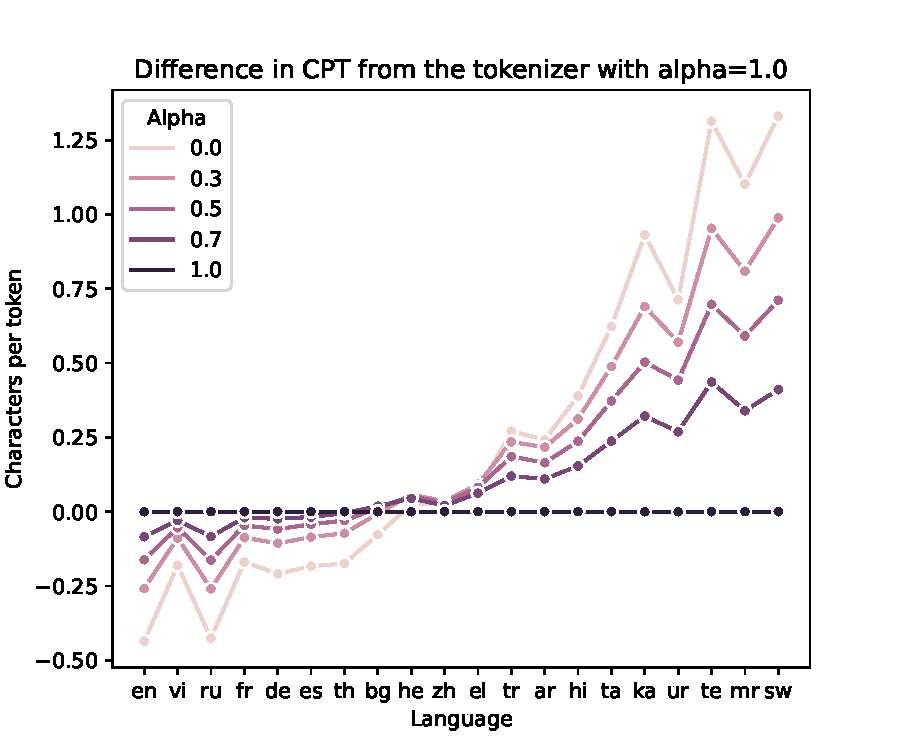
\includegraphics[width=\textwidth]{img/results/cpt_vs_alpha.pdf}
    \caption{We examine the impact of the language imbalance on the Sentencepiece Unigram tokenizer training. We train five tokenizers with an increasing language imbalance controlled by the $\alpha$ parameter. Then we look at the effect on the vocabulary allocation metrics per language. We center the results using the most unbalanced tokenizer with $\alpha=1.0$. As expected, the more balanced tokenizers have higher vocabulary allocation scores for low resource languages and lower scores for high resource languages. Interestingly, the effect varies across languages. For example the vocabulary allocation of high-resource Vietnamese or French is not as affected by the decrease in training data as English or Russian. \xxx{We also observe that the data imbalance negatively affects the low resource languages more than it positively affects the high resource languages. This suggests that the marginal benefit of adding more data to the high resource languages is lower than the incurred cost on the quality of tokenization for the low resource languages. <- is this a good interpretation?}}
    \label{fig:data_balance_vs_allocation_per_lang}
\end{figure}


\section{Comparison of balancing methods}
\subsection{Balancing methods and vocabulary allocation}

\begin{table}
\caption{In this summary table, we present all tokenizers used in this chapter. Along with the Huggingface tokenizers from table \ref{fig:20l_metrics} and Sentencepiece Unigram tokenizers from \ref{fig:data_balance_vs_allocation_per_lang}, we include the tokenizers obtained by replicating the papers \citet{chung_improving_2020,zheng_allocating_2021,liang_xlm-v_2023} in our setting. As we can see, the Huggingface Unigram tokenizer is a clear outlier in terms of all metrics even after taking account the higher alphabet size as explored in \ref{tab:coverage_influence}. Further we can see that the proposed balancing methods are improving over the baselines the authors used (\textit{unigram\_alpha0.5} and \textit{unigram\_alpha0.7}). On the other hand we see that using more balanced data for training the Sentencepiece Unigram (\textit{unigram\_alpha0.0}) does lead to similar overall performance as the replicated methods.
The rows are sorted by the CPT score. \xxx{As we can see that except for the Huggingface tokenizers, the alphabet sizes for all tokenizers stay in the stable range of 1000-5000. This corresponds to a comparable number number of UNKs in the holdout data.
}}
\label{tab:all_tokenizers_metrics}
\begin{tabular}{lrrrrr}
\toprule
Tokenizer & Alphabet & \# UNKs & CPT & AR & JSD \\
\midrule
huggingface\_bpe\_alpha0.25 & 1000 & 14040.1 & 3.713 & 1253.7 & 0.783 \\
unigram\_alpha0.0 & 2975 & 617.1 & 3.712 & 1212.9 & 0.767 \\
Chung\_20clusters & 4123 & 270.3 & 3.702 & 1098.7 & 0.766 \\
unigram\_alpha0.3 & 2666 & 923.5 & 3.702 & 1190.7 & 0.768 \\
TokMix\_alpha0.25 & 2497 & 1203.2 & 3.691 & 1163.4 & 0.773 \\
Chung\_16clusters & 3933 & 387.1 & 3.677 & 1102.2 & 0.767 \\
Liang\_20clusters & 3709 & 341.4 & 3.676 & 1103.2 & 0.765 \\
Zheng\_20langs & 4854 & 245.7 & 3.673 & 1094.5 & 0.765 \\
Liang\_16clusters & 3655 & 416.8 & 3.669 & 1106.2 & 0.767 \\
bpe\_alpha0.25 & 1215 & 7235.6 & 3.666 & 1212.9 & 0.774 \\
unigram\_alpha0.5 & 2859 & 729.0 & 3.618 & 1143.8 & 0.769 \\
Chung\_8clusters & 4870 & 684.4 & 3.575 & 1061.1 & 0.770 \\
unigram\_alpha0.7 & 2733 & 883.2 & 3.556 & 1107.1 & 0.770 \\
Chung\_4clusters & 3253 & 648.6 & 3.546 & 1071.9 & 0.768 \\
Liang\_8clusters & 4283 & 568.2 & 3.544 & 1081.6 & 0.767 \\
Liang\_4clusters & 3698 & 419.2 & 3.512 & 1082.5 & 0.769 \\
unigram\_alpha1.0 & 2476 & 1286.3 & 3.442 & 1041.8 & 0.772 \\
huggingface\_unigram\_alpha0.25 & 12616 & 4.5 & 3.204 & 1010.5 & 0.745 \\
\bottomrule
\end{tabular}
\end{table}


\begin{figure}[H]
    \centering
    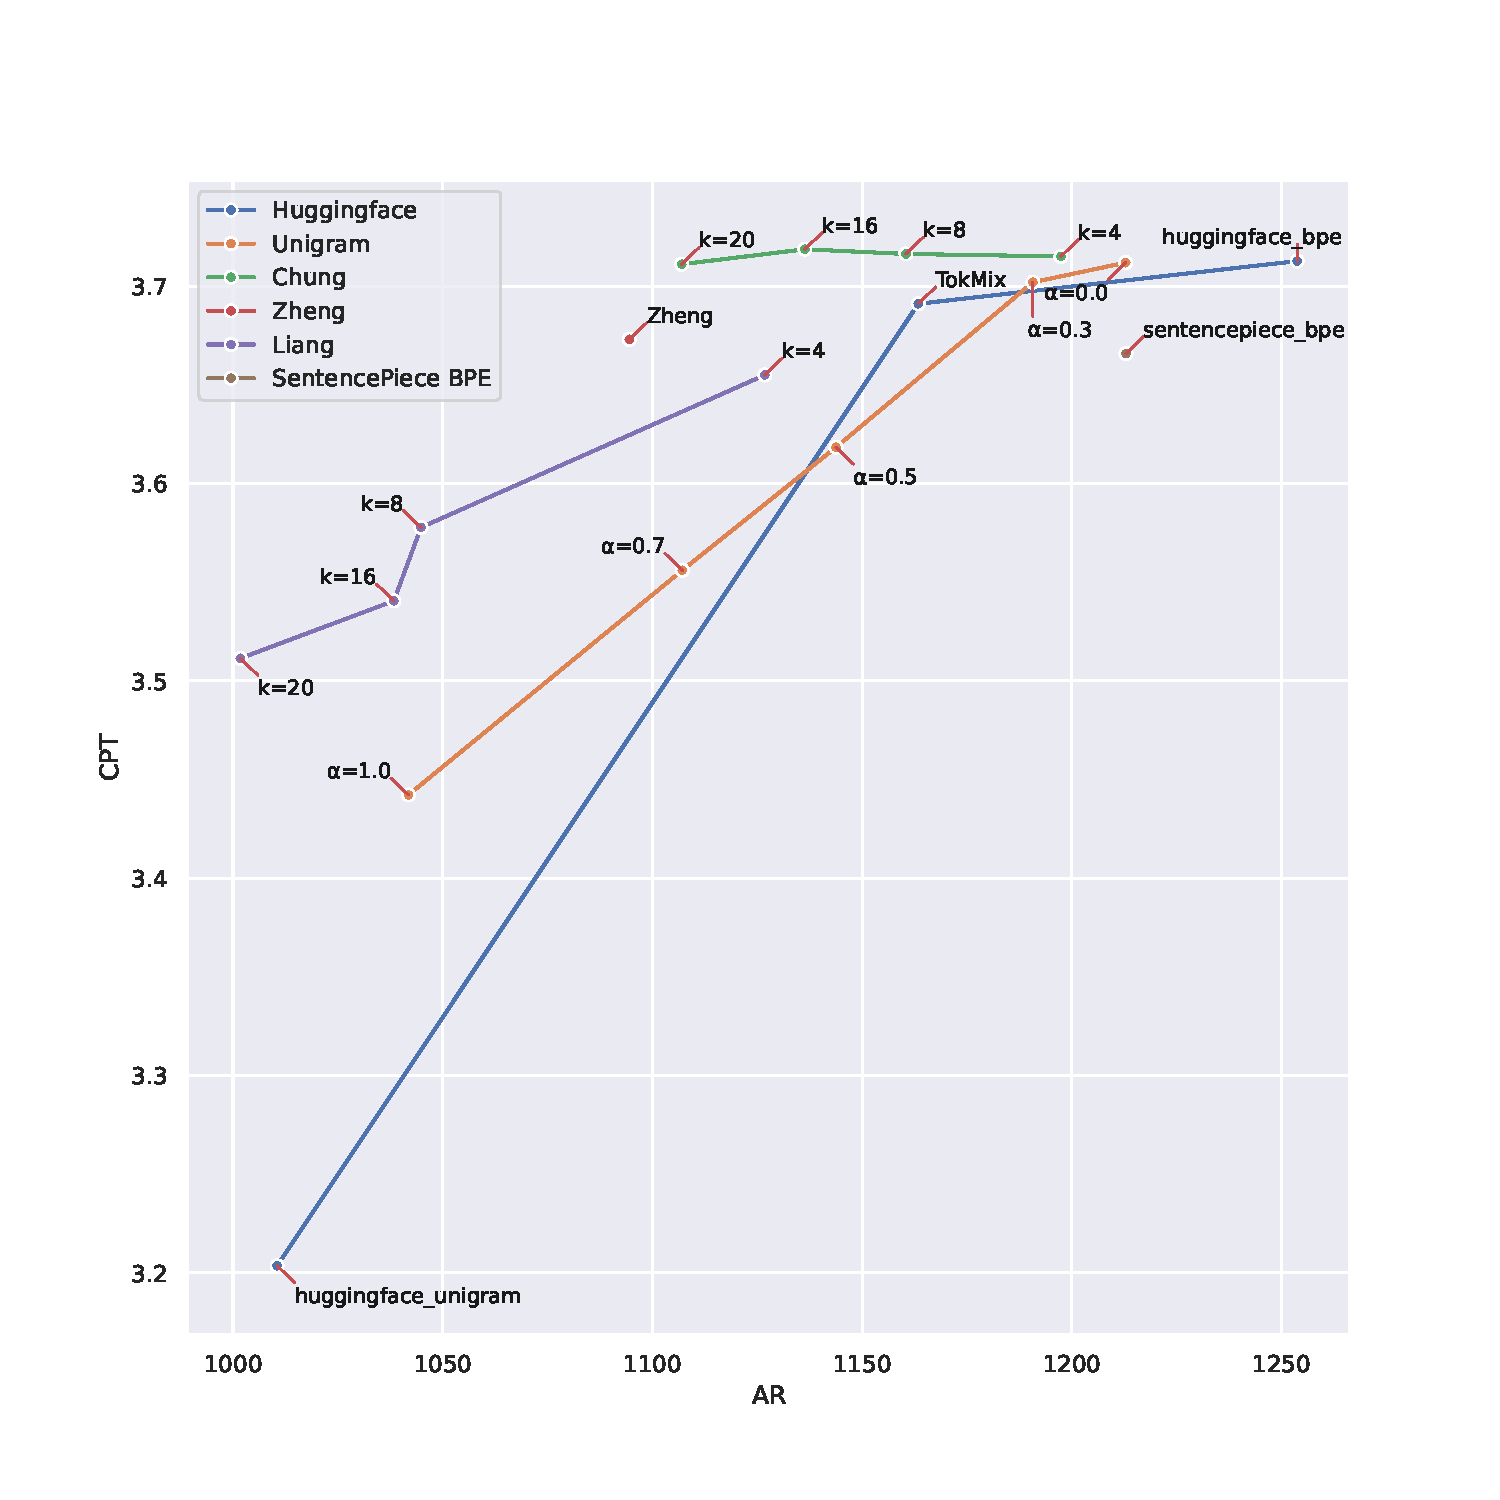
\includegraphics[width=\textwidth]{figures/all_tokenizers_AR_vs_CPT.pdf}
    \caption{We visualize the overall vocabulary allocation metrics for all tokenizers from Table \ref{tab:all_tokenizers_metrics}. We observe that the vocabulary allocation scores are related --- higher AR usually means higher CPT. Nevertheless, we also have tokenizers with low AR and high CPT but never the other way around. Our intuition is that it is not possible to construct a tokenizer with high number of useful tokens which are all very short. We also observe that Huggingface Unigram is a clear outlier, although combination of separate, monolingual Huggingface Unigrams (TokMix) approaches the performance of the Sentencepiece Unigram with the corresponding data imbalance ($\alpha=0.3$). We again see, that the balancing methods, especially Chung and Zheng overperform the unbalanced baselines ($\alpha=0.7$, $\alpha=0.5$) but perform similarly or worse to the simple case of running the Sentencepiece Unigram trainer on a balanced set $\alpha=0.0$.}
    \label{fig:all_tokenizers_AR_vs_CPT}
\end{figure}

\begin{figure}[H]
    \centering
    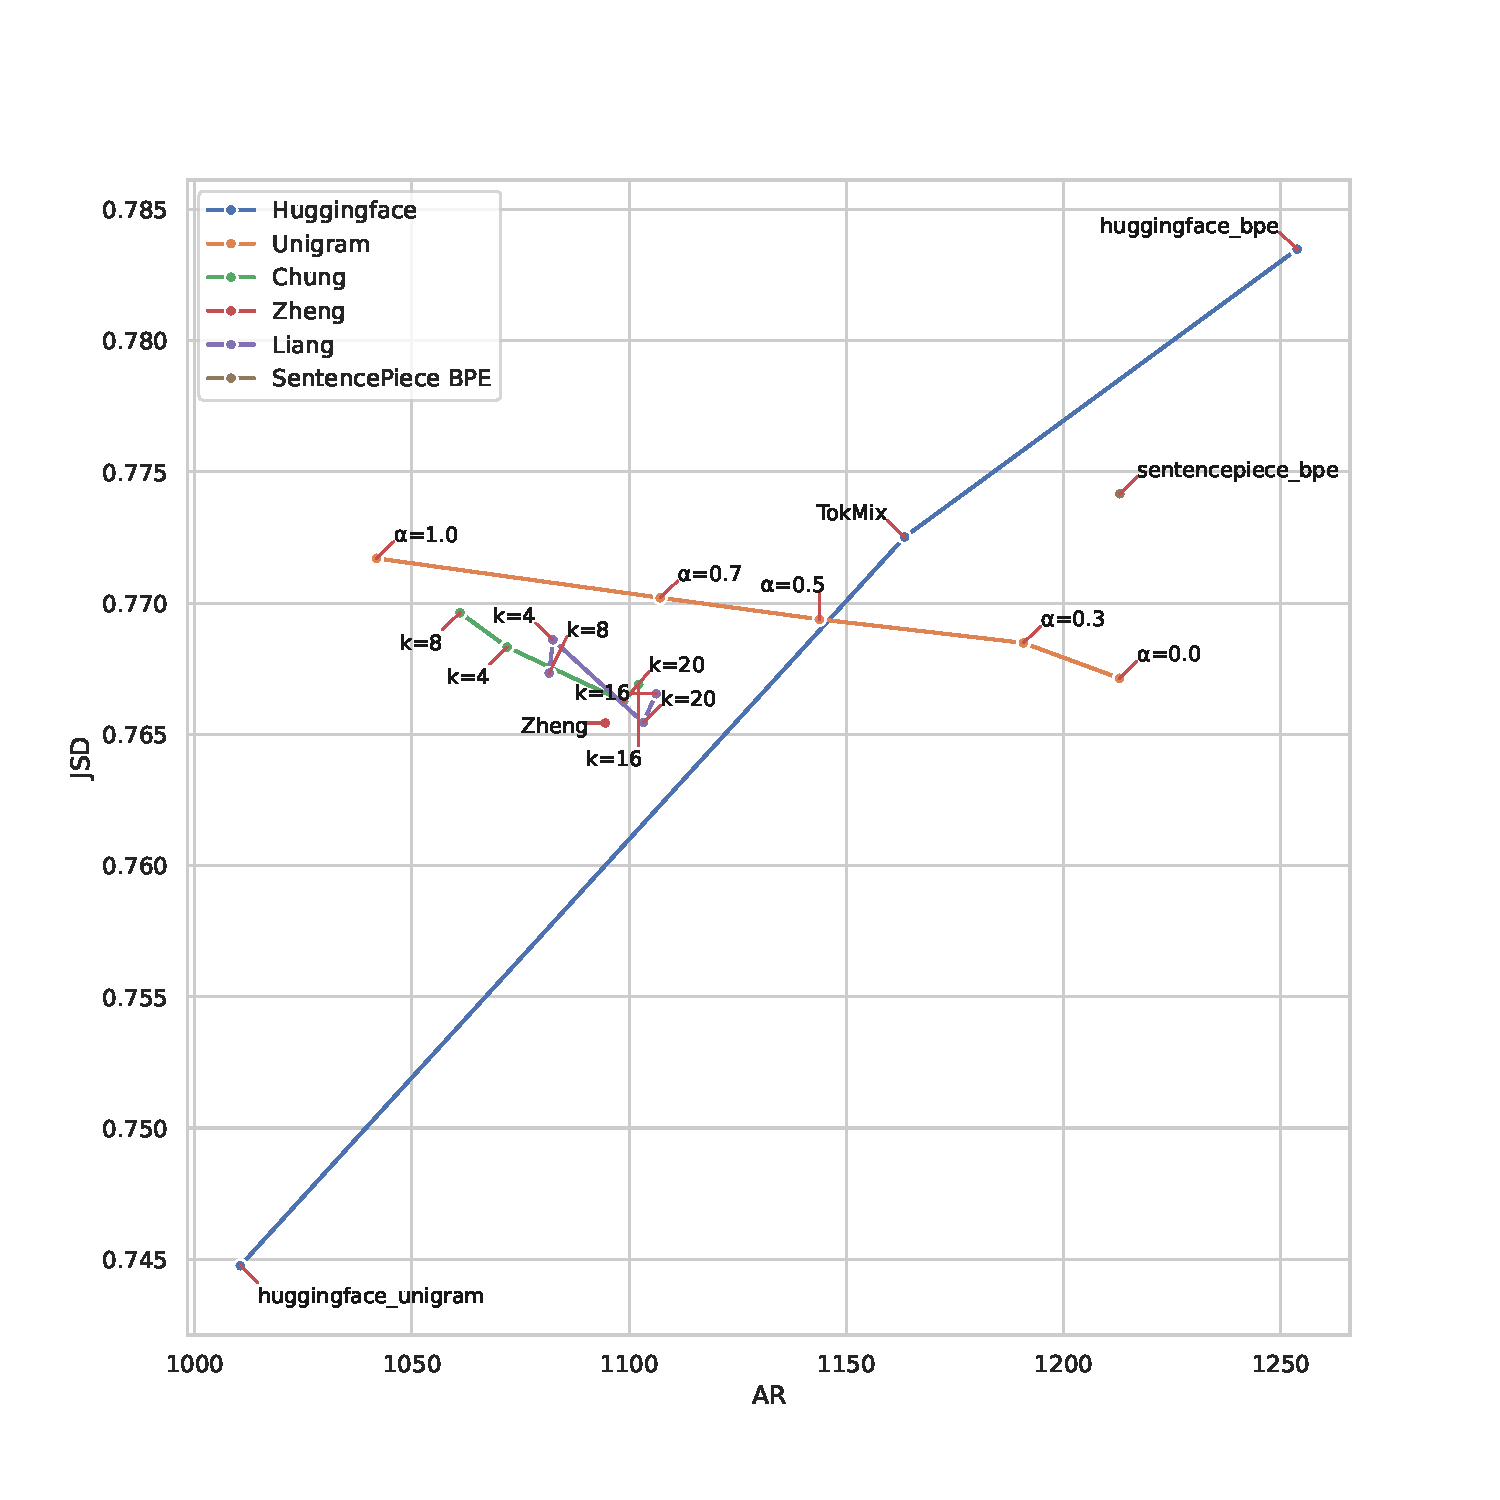
\includegraphics[width=\textwidth]{figures/all_tokenizers_AR_vs_JSD.pdf}
    \caption{We visualize the tokenizers from Table \ref{tab:all_tokenizers_metrics} in terms of Average Rank and Jensen-Shannon Divergence. Here we can see that all methods based on Sentencepiece result in similar overlap independent of the allocation. This is interesting because the replicated balancing methods (Chung, Zheng, Liang) work by splitting the data and training separate tokenizers. Nevertheless, after merging the separate subtokenizers they all seem to end up with similar vocabulary overlaps. The highest vocabulary isolation is surprisingly achieved by the Huggingface BPE tokenizer, which is contrary to the hypothesis stated by \citet{chung_improving_2020,zheng_allocating_2021} that the tokenizers trained on the concatenation of all data tend to select subwords shared across all languages.}
    \label{fig:all_tokenizers_AR_vs_JSD}
\end{figure}

\begin{figure}[H]
    \centering
    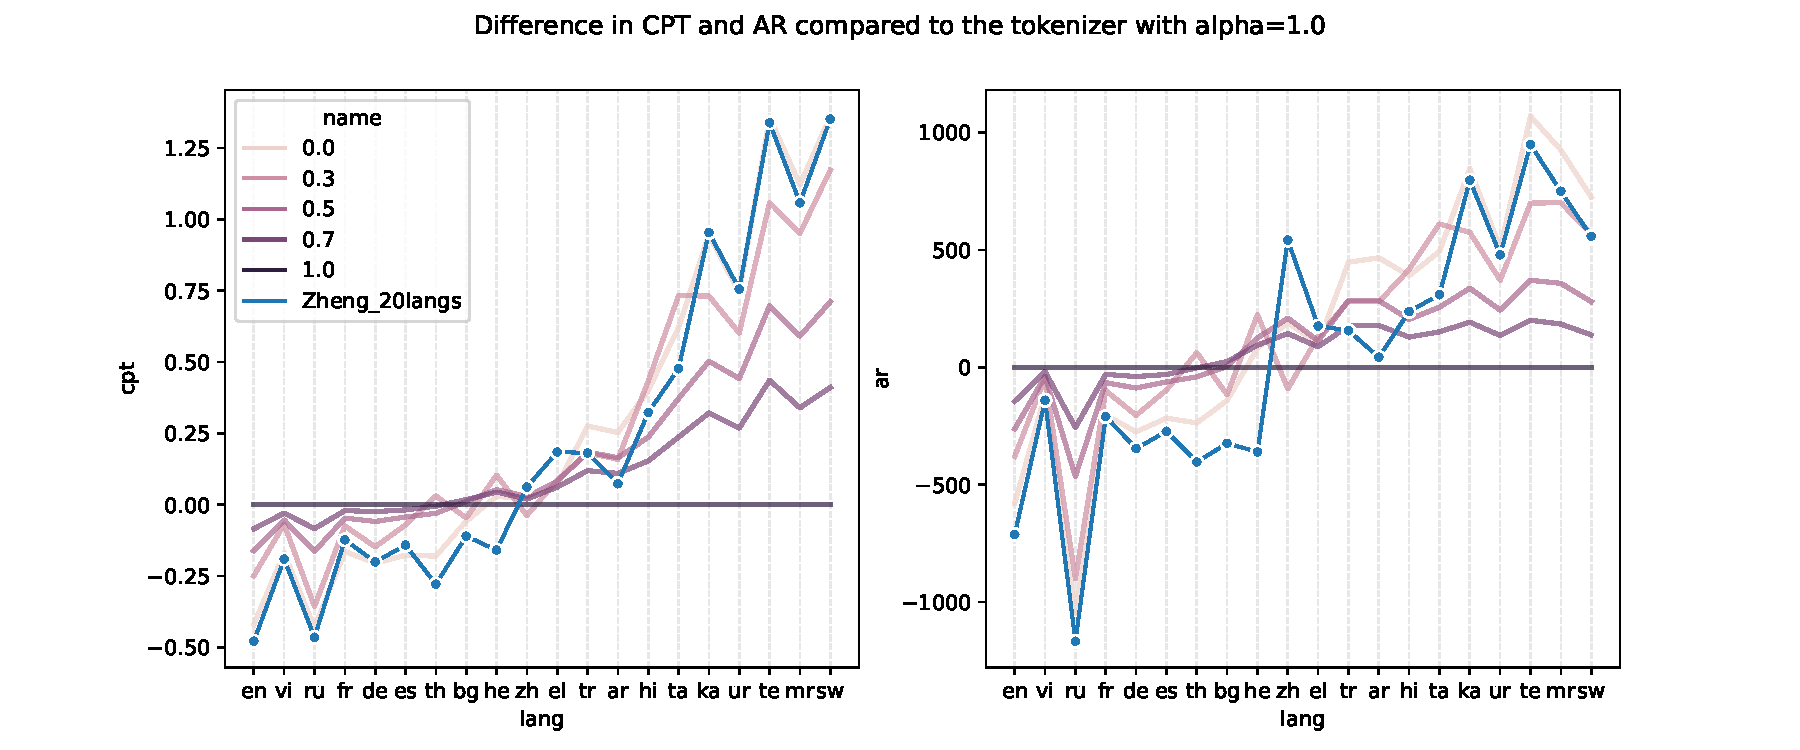
\includegraphics[width=\textwidth]{figures/zheng_vs_alphas.pdf}
    \caption{We zoom into the results of the Zheng method and compare the vocabulary allocation across the individual languages represented by this tokenizer against the backdrop of the vanilla Unigram tokenizers trained with different data imbalances from \ref{fig:data_balance_vs_allocation_per_lang}. We observe a striking similarity between the vocabulary allocation of the Zheng tokenizer and the Unigram tokenizer with $\alpha=0.0$, especially in terms of characters per token. This comes as a large surprise because the Zheng method works by training a separate tokenizer for each language and then merging them together. Despite the different method of obtaining the vocabulary, the resulting tokenizers are very similar across the languages.}
    \label{fig:zheng_vs_alphas}
\end{figure}

\begin{figure}[H]
    \centering
    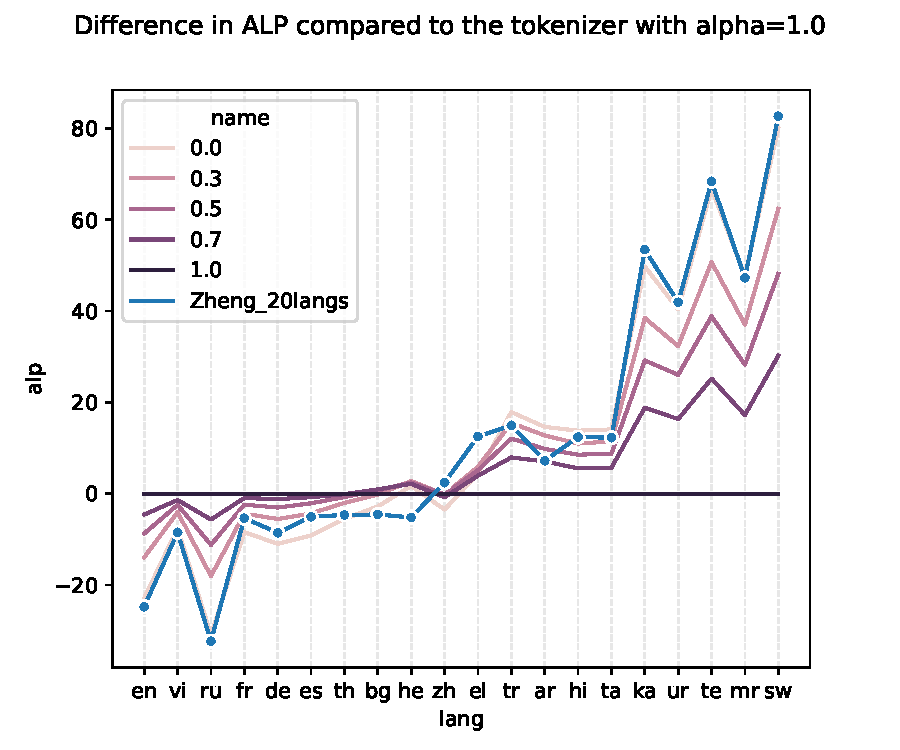
\includegraphics[width=\textwidth]{figures/zheng_vs_alphas_alp.pdf}
    \caption{Intrigued by the similarity between the Zheng tokenizer and the Unigram tokenizer with $\alpha=0.0$ from Figure \ref{fig:zheng_vs_alphas} we also look at the ALP metric which is used for the selection of vocabulary sizes in the Zheng method. Here we see that the greedy optimization of ALP across languages indeed results in a similar vocabulary allocation as the Unigram tokenizer with $\alpha=0.0$.}
    \label{fig:zheng_vs_alphas_alp}
\end{figure}



\begin{figure}[H]
    \centering
    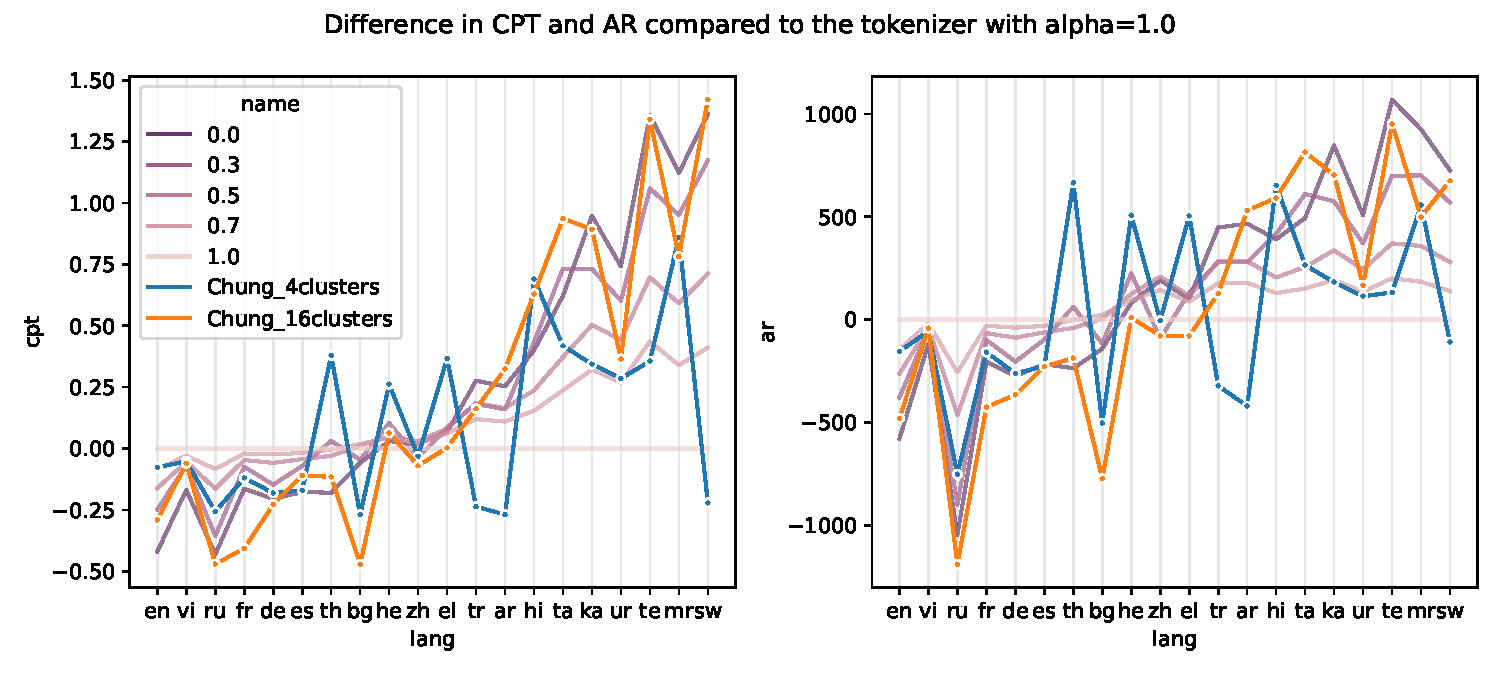
\includegraphics[width=\textwidth]{figures/chung_vs_alphas.pdf}
    \caption{Here we inspect the language-level vocabulary allocation of the Chung method. Similarly to the Zheng method, the Chung method also performs similarly to the Unigram tokenizer with $\alpha=0.0$. Unfortunately, we believe this is an artifact of the choice of our training data for the Chung method. We use a balanced dataset ($\alpha=0.0$) for training the cluster-specific tokenizers. The balance of the data seems to be more important than the clustering step. After merging the cluster-specific tokenizers, the resulting tokenizer is very similar to the Unigram tokenizer with $\alpha=0.0$.}
    \label{fig:chung_vs_alphas}
\end{figure}

\begin{figure}[H]
    \centering
    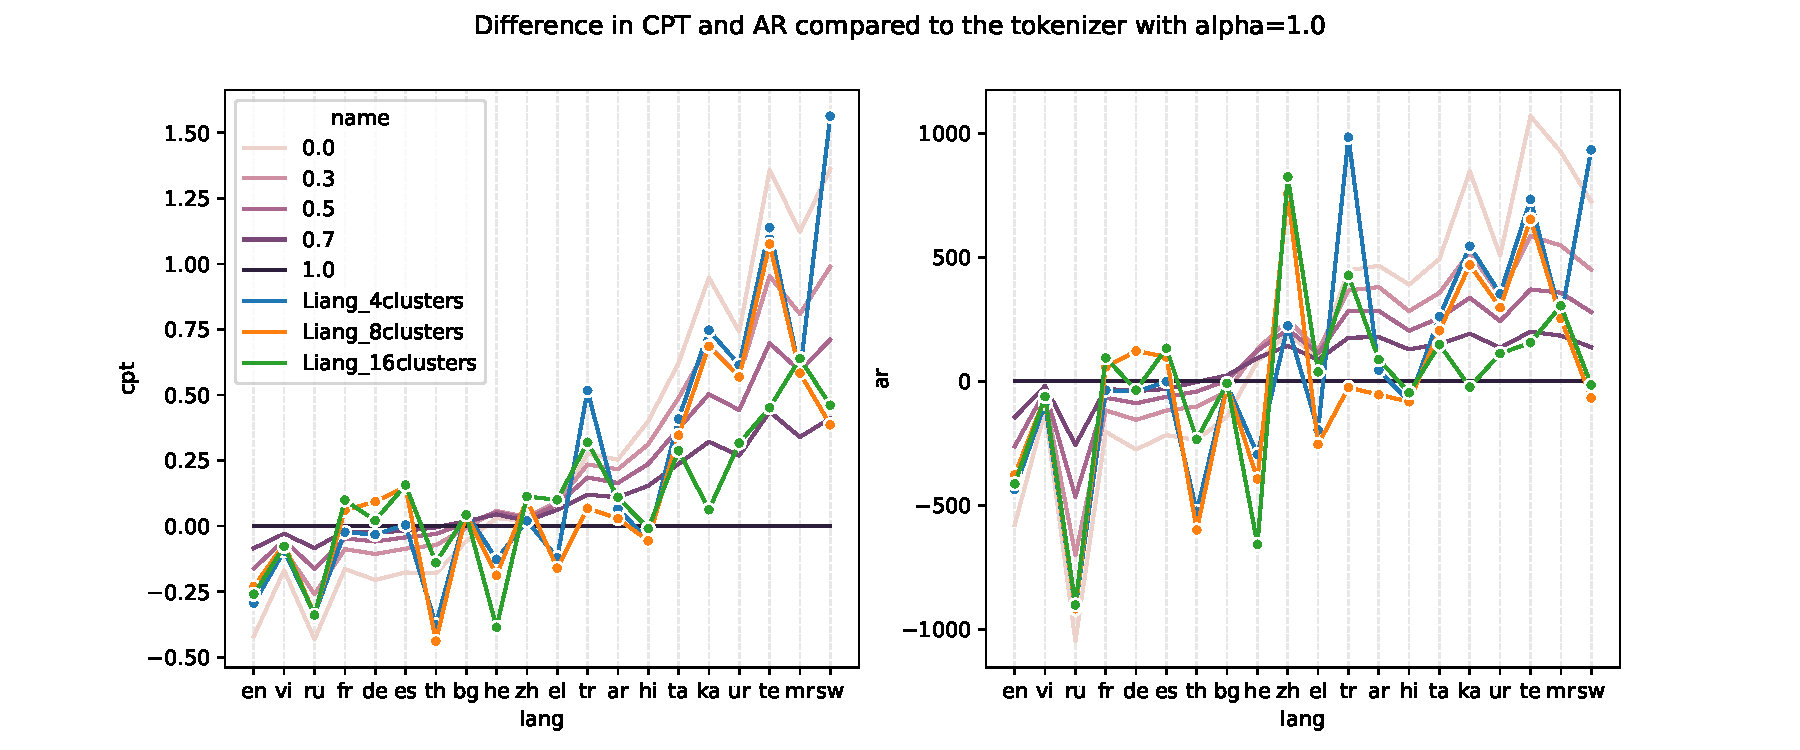
\includegraphics[width=\textwidth]{figures/liang_vs_alphas.pdf}
    \caption{Interestingly, the Liang method seems to yield the most distinct results despite the fact it is trained with balanced data and uses the greedy allocations from the Zheng method. \xxx{TODO: explain why}}
    \label{fig:liang_vs_alphas}
\end{figure}

\subsection{Balancing methods and vocabulary overlap}
\section{Comparison of balancing methods on downstream tasks}


\begin{figure}
    \centering
    \begin{subfigure}{.5\textwidth}
      \centering
      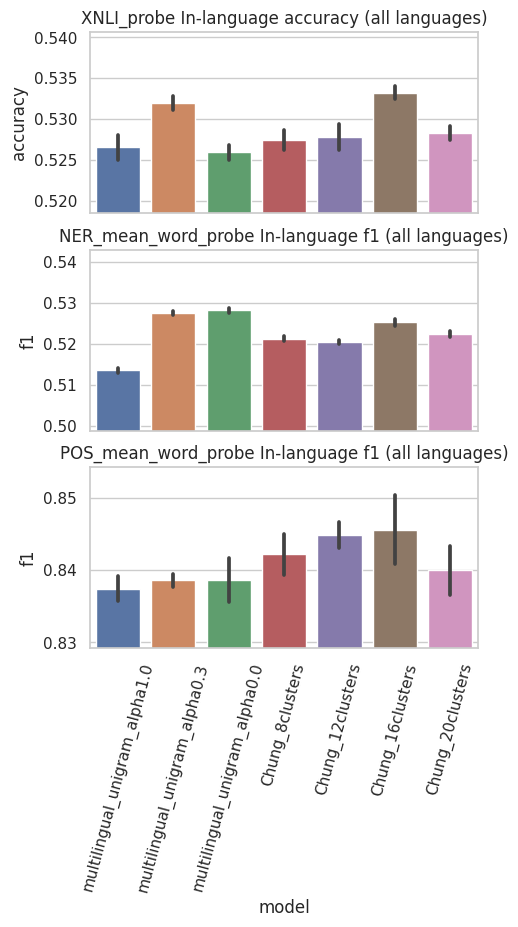
\includegraphics[width=\linewidth]{img/temp/probe_overall_inlanguage.png}
      \caption{In-language results}
      \label{fig:probe_overall_inlanguage}
    \end{subfigure}%
    \begin{subfigure}{.5\textwidth}
      \centering
      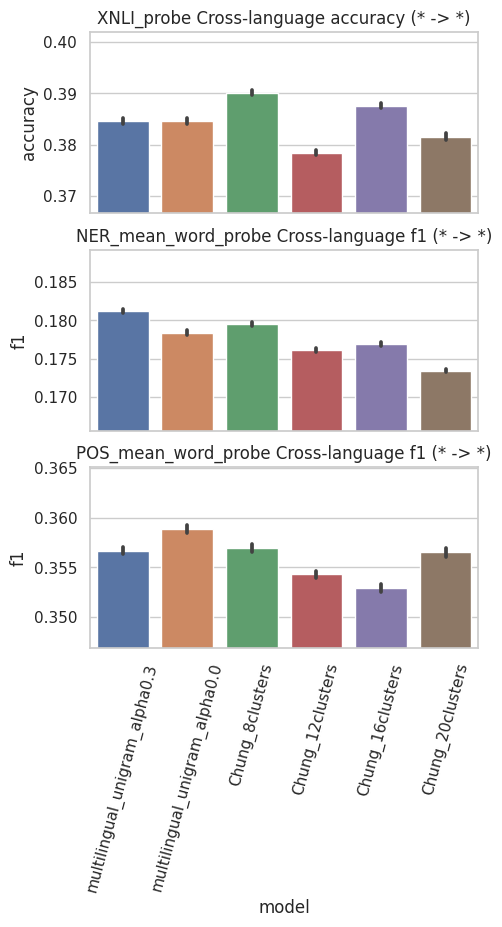
\includegraphics[width=\linewidth]{img/temp/probe_overall_crosslanguage.png}
      \caption{Cross-language results}
      \label{fig:probe_overall_crosslanguage}
    \end{subfigure}
    \caption{We select the best performing balancing method by \citet{chung_improving_2020} from our replications based on our tokenizer metrics and compare it with the vanilla Unigram tokenizers. We choose the unbalanced Unigram tokenizer with $\alpha=1.0$ and then two stronger baselines with $\alpha=0.0$ and $\alpha=0.3$ trained on more balanced data. We then pretrain masked language models that differ only in the tokenizer they use and assess the performance of these models on the downstream tasks using probing. We test two settings --- in-language performance, where the model is trained on each of the available languages and then evaluated on the same language, and cross-language performance, where the model is also trained on each language but evaluated on all \textit{but} the training language. We observe that for word-level tasks all balanced tokenizers (where $\alpha\neq1.0$) perform significantly better than the unbalanced Unigram. Moreover we see that the differences between the individual balancing methods seem to be minimal. For sentence-level NLI, we do not observe any systematic effects as the differences between the runs are quite low (<1\% accuracy).
    The results are a macro average over all the languages (in-language results) or language pairs (cross-language results). For each model and language we do 3 probe training runs with different random seeds. The error bars represent one standard deviation computed with bootstrapping by randomly sampling seeds for each language. Note that even though the probe training is done with three different random seeds, the model pretraining was done only once. The variance between pretraining runs is therefore not measured and the error bars should be interpreted as such.}
    \label{fig:probe_overall}
\end{figure}

% \begin{figure}[H]
%     \centering
%     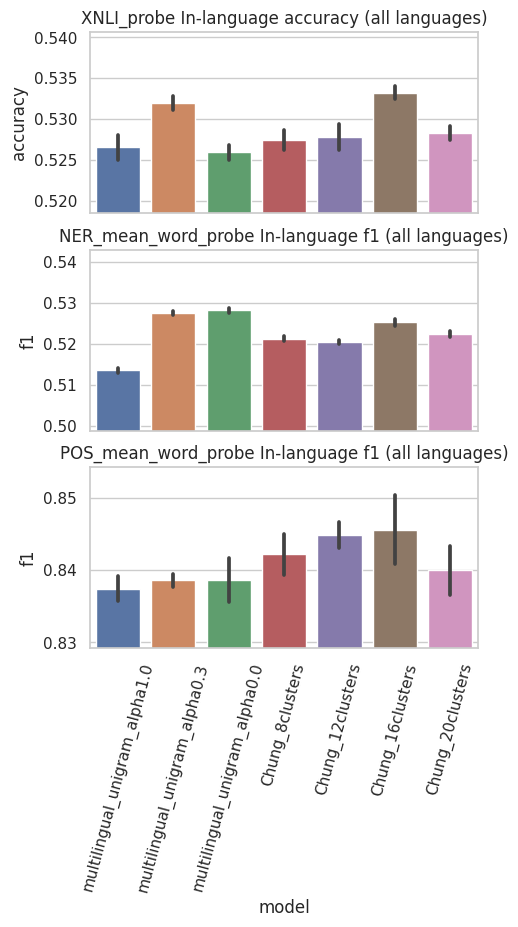
\includegraphics[width=\textwidth]{img/temp/probe_overall_inlanguage.png}
%     \caption{probe overall inlanguage}
%     \label{fig:probe_overall_inlanguage}
% \end{figure}


\begin{figure}[H]
    \centering
    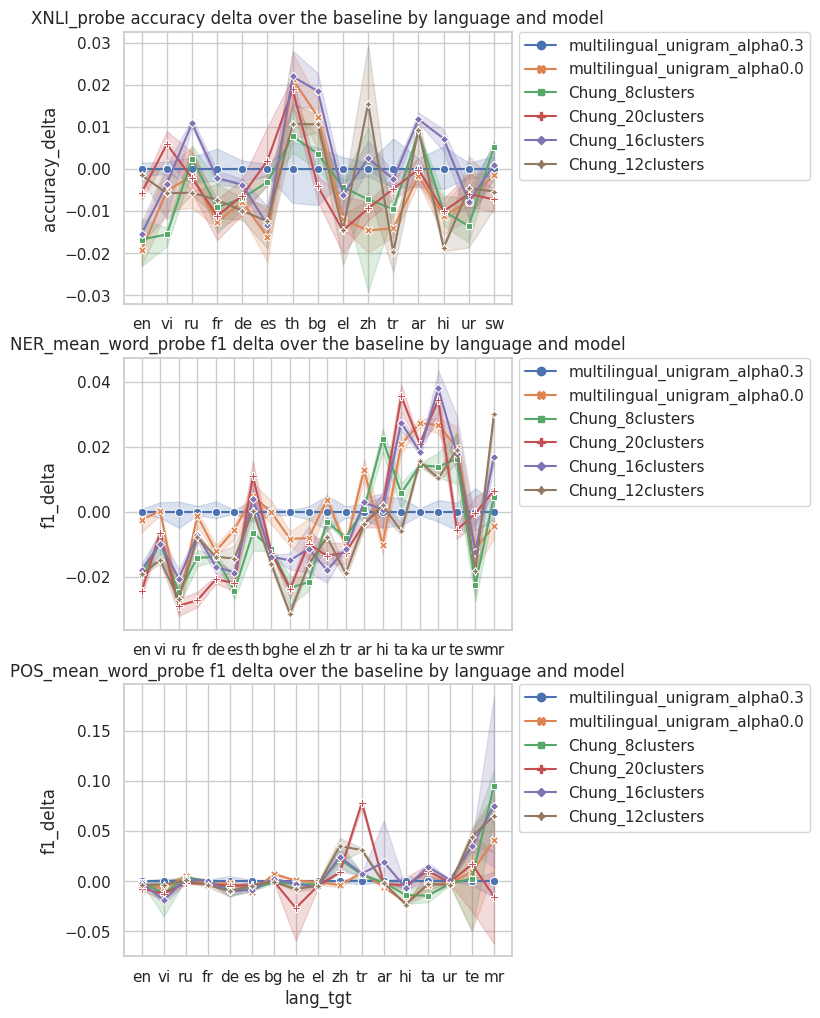
\includegraphics[width=\textwidth]{img/temp/probe_overall_inlanguage_over_baseline.png}
    \caption{We zoom in on the in-language results from Figure \ref{fig:probe_overall_inlanguage} and compare the performance of the balanced tokenizers against the unbalanced Unigram tokenizer with $\alpha=1.0$ over all tested languages for the tasks. In case of the word-level tasks, especially in the case of named entity recognition, we observe a clear trend in line with our tokenizer investigations in \ref{fig:chung_vs_alphas}. The balancing methods improve the language representations for the word-level tasks. For the sentence-level tasks, we do not observe any systematic effects. This might be in part due to the fact that the NLI task does not include 4 of our low-resource languages. The error bands are one standard deviation computed from the three probe training runs with different random seeds.}
    \label{fig:probe_overall_inlanguage_over_baseline}
\end{figure}


\begin{figure}[H]
    \centering
    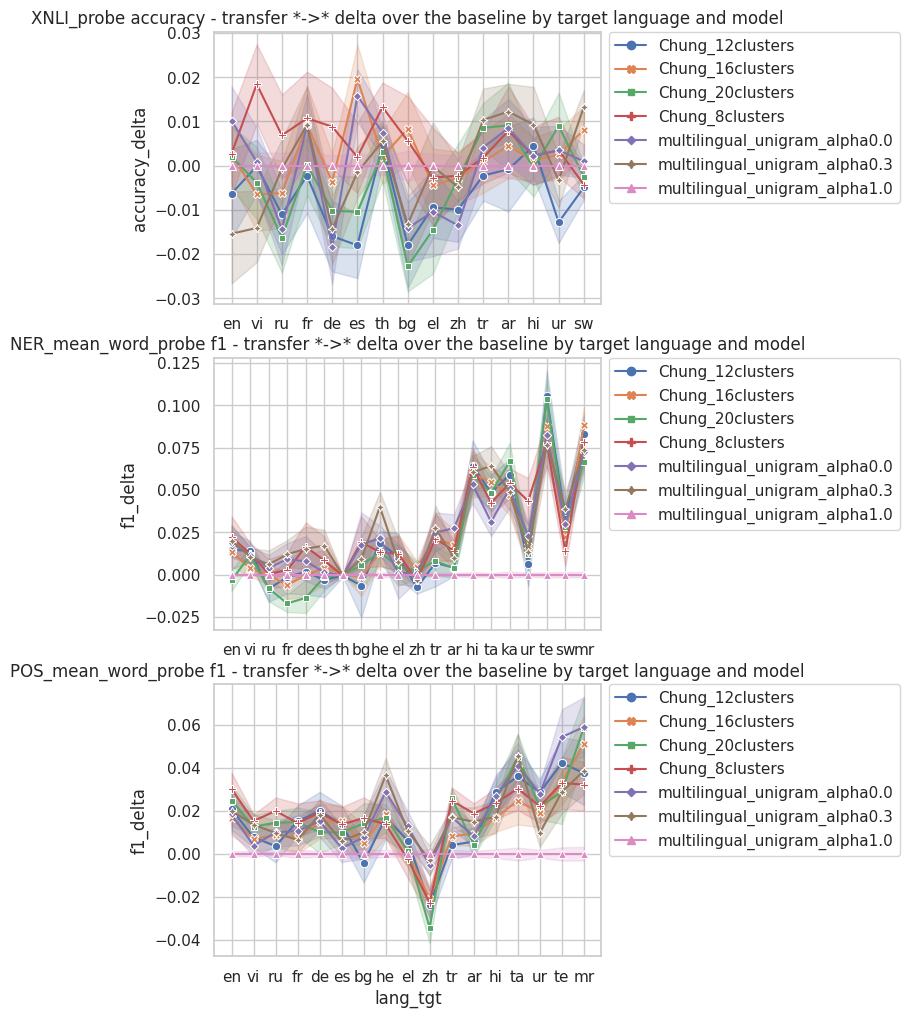
\includegraphics[width=\textwidth]{img/temp/probe_overall_crosslanguage_over_baseline.png}
    \caption{Here we investigate in detail the cross-lingual results from Figure \ref{fig:probe_overall_crosslanguage} with comparison to the unbalanced Unigram tokenizer with $\alpha=1.0$. We observe that word-level task transfers behave in line with the tokenizer investigations in \ref{fig:chung_vs_alphas}. Moreover it seems that both high-resource and low-resource languages benefit from the balancing methods, although the change is most clear at the low-resource side. For the sentence-level tasks, we do not observe any systematic effects.}
    \label{fig:probe_overall_crosslanguage_over_baseline}
\end{figure}



\begin{figure}[H]
    \centering
    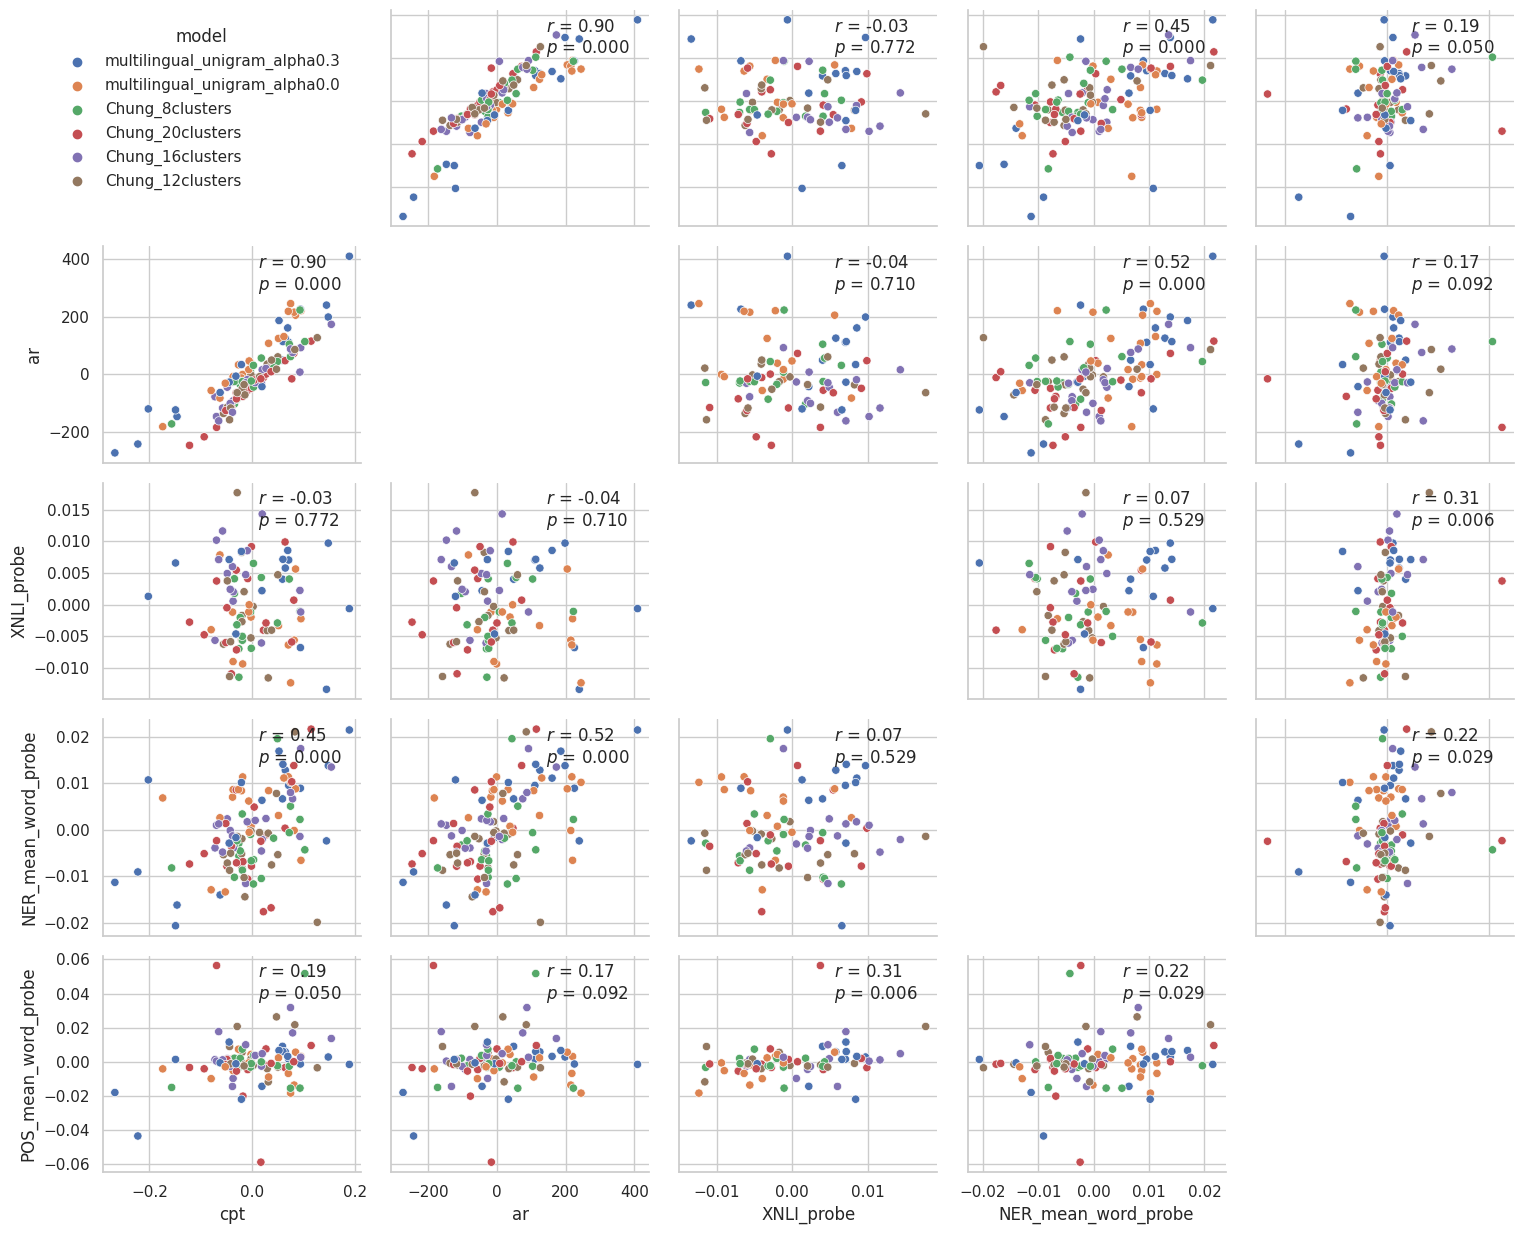
\includegraphics[width=\textwidth]{img/temp/probe_overall_inlanguage_scattermatrix.png}
    \caption{We visualize the in-language results from Figure \ref{fig:probe_overall_inlanguage} in a scatter matrix. We center the results for each language and then plot the differences from mean performance against the differences in our tokenizer metrics. We see significant spearman correlations for the NER and POS tasks, although for POS the correlation is low. For the NLI task, we do not observe any significant correlations.}
    \label{fig:probe_overall_inlanguage_scattermatrix}
\end{figure}


% \begin{figure}[H]
%     \centering
%     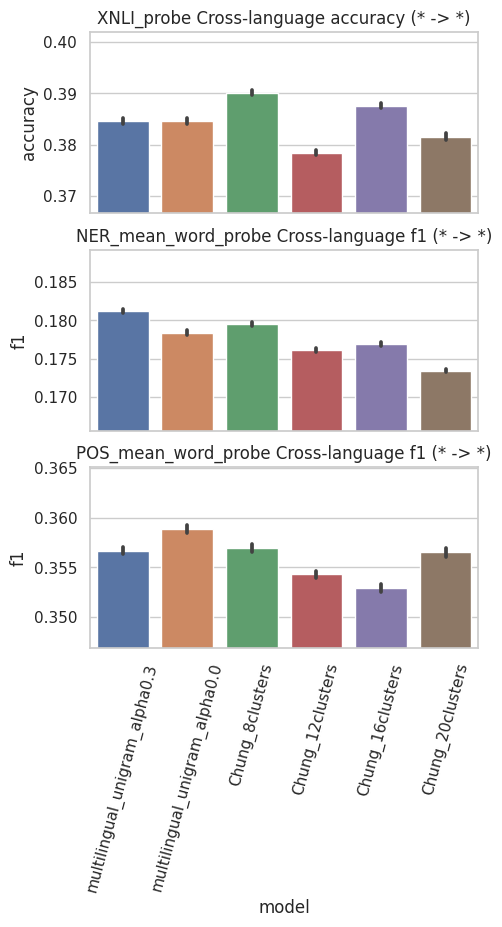
\includegraphics[width=\textwidth]{img/temp/probe_overall_crosslanguage.png}
%     \caption{probe overall crosslanguage}
%     \label{fig:probe_overall_crosslanguage}
% \end{figure}

\begin{figure}[H]
    \centering
    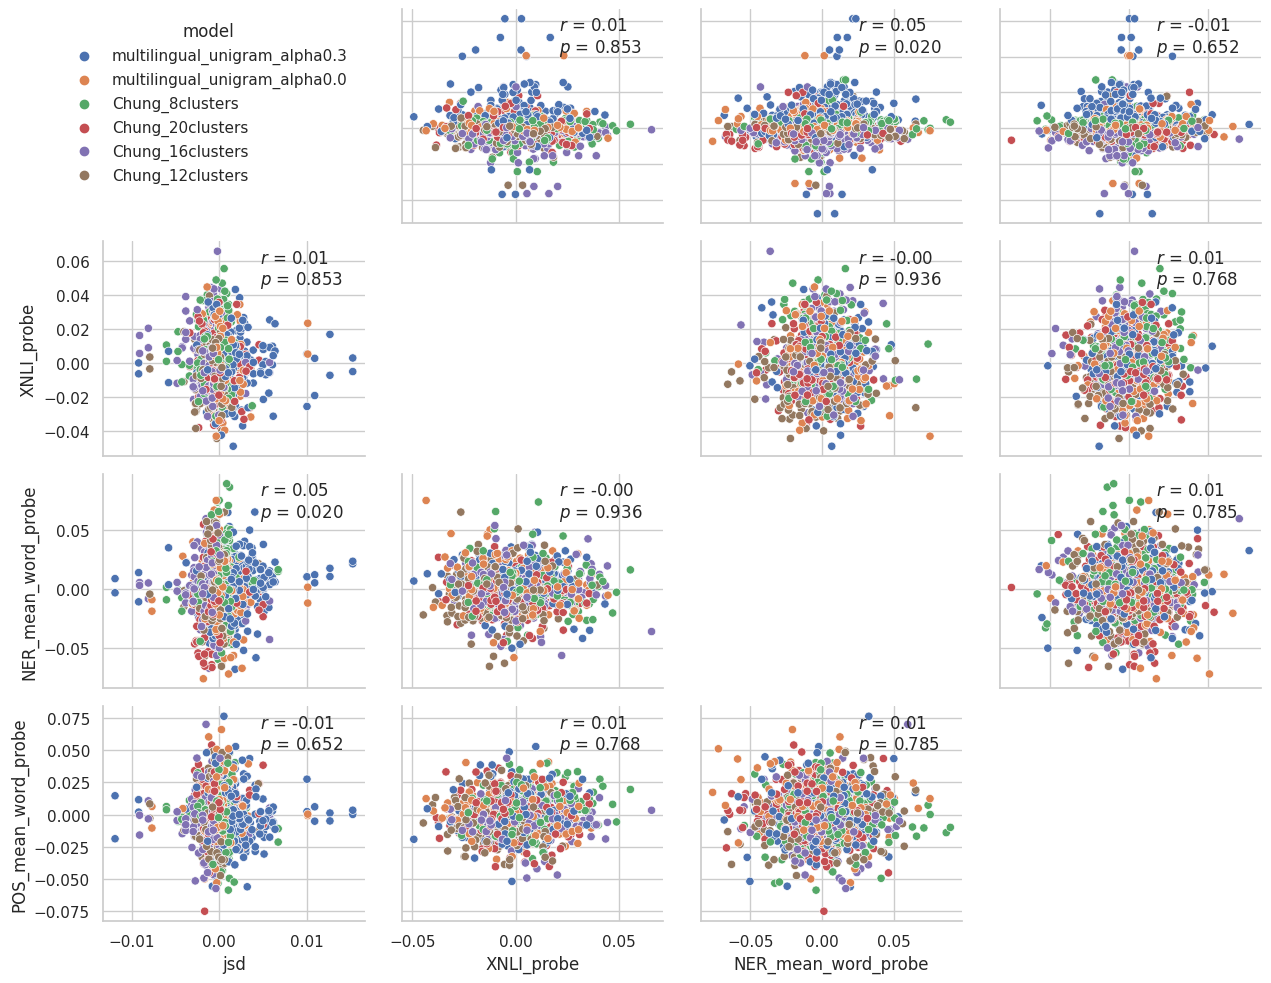
\includegraphics[width=\textwidth]{img/temp/probe_overall_crosslanguage_scattermatrix.png}
    \caption{We visualize the cross-language results from Figure \ref{fig:probe_overall_crosslanguage} in a scatter matrix. We center the results for each language and then plot the differences from mean performance against the differences in the vocabulary overlap metric (JSD). We see significant, very low negative correlation for the NER and POS tasks. This might suggest that the word-level tasks benefit only very slightly from an increase in overlap (decrease in JSD). For the NLI task, we do not observe any significant correlations.}
    \label{fig:probe_overall_crosslanguage_scattermatrix}
\end{figure}

% visualization idea:

% - visualization of tokenizer balance difference is too noisy to see the differences between methods
%     - smoothing num_lines_per_language vs cpt
%     - or fitting a line
%     - something that highlights if one balancing method is better than another

% \section{Preliminary experiments}
% \subsection{The importance of training data size}
% \subsection{Differences in tokenizer implementations}
% \section{Reproduction of baselines}
% \section{Document-level clustering method}
% \section{Extrinsic evaluation}


% - replication of the previous work
%     - Chung
%         - reproductions in Overlap-based Vocabulary Generation Improves Cross-lingual Transfer Among Related Languages

%     - Liang
%         - they use 900k vocab, they compare their model to XLM-R which is not fair!
%             - they discuss it in section 6.4
%         - reproductions: https://github.com/stefan-it/xlm-v-experiments
%             - For XQuAD they did not reproduce the improvements
%             - For MasakhaNER they reproduced the improvements
%             - TODO: could use bootstrapping to show whether the improvements are significant

% replications of Chung, Liang
% https://github.com/stefan-it/xlm-v-experiments

% - our beta experiments point to the randomness of the output - the smooth sweep across the beta values seems to produce quite noisy outpus
